\documentclass{beamer}

\usepackage{mathpazo}
\usepackage[english]{babel}
\usepackage{kotex}
\usepackage{epstopdf}
\usepackage{wallpaper}
\usepackage{mdframed}
\usepackage{geometry}
\usepackage{amsthm}
\usepackage{amsmath}
\pdfmapfile{+sansmathaccent.map}

%%
\usetheme{ENSLyon} %http://mike.depalatis.net/beamerthemes/
%\useoutertheme[footline=authorinstitutetitle]{miniframes}
\title[Title]{A Study on Comparison of\\ Bayesian Network Structure Learning Algorithms\\ for Selecting Appropriate Models}
\author[Joe]{Jae-seong Yoo}
\institute[]{Dept. of Statistics}
%\date{\today}
\date{December 5, 2014}
  \setbeamersize{text margin left=5mm}
  \setbeamersize{text margin right=5mm}


% pour supprimer les symboles de navigation
\setbeamertemplate{navigation symbols}{}
\usecolortheme{ENSLyon_blue}



\begin{document}

\begin{frame}
	\titlepage
{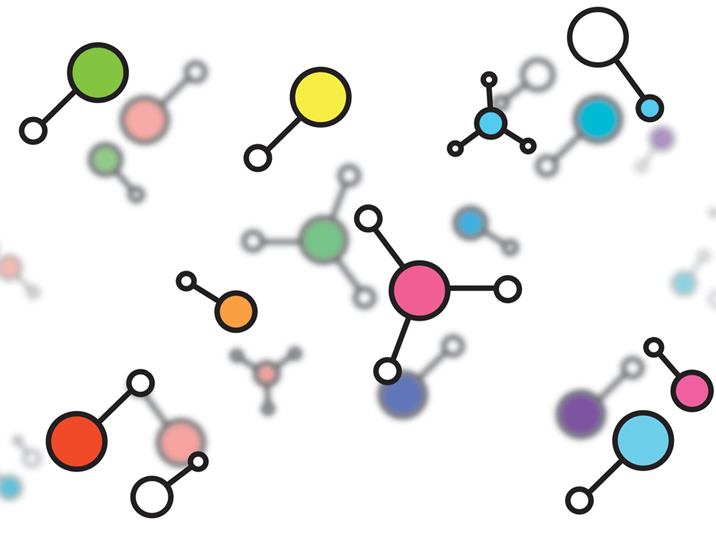
\includegraphics[	width=\paperwidth,
								height=\paperheight,keepaspectratio]
								{background.jpg}}
\end{frame}


\begin{frame}
\frametitle{Title}
{\scriptsize{}
	\tableofcontents
}
\end{frame}


\section{Introduction}
\subsection{Goal}
\begin{frame}
\frametitle{Goal}
{\scriptsize{}
\begin{itemize}
	\item In this paper, we \textcolor{red}{compare the performance} between the Bayesian network \textcolor{red}{structure learning algorithms} provided by \textbf{bnlearn} package in \textbf{R}.

	{}\
	
	\item The performance is \textcolor{red}{evaluated} by

	\begin{itemize}
		\item \textcolor{red}{using a score}
		
		 or
		 
		\item comparing between the \textcolor{red}{target network} and the \textcolor{red}{learnt network}.
	\end{itemize}	
	
		In this paper, it was confirmed that algorithm specific performance test results using fore-mentioned methods are different.

	{}\

	\item A \textcolor{red}{data generator} based on Bayesian network model using \textbf{R} is built and introduced.

	{}\

	\item The aim of this paper is to provide objective guidance of selecting suitable algorithm in accordance to target network \textcolor{red}{using synthetic data generated based on topology}.
\end{itemize}
}
\end{frame}


\subsection{Bayesian Network}
\begin{frame}
\frametitle{Bayesian Network}
{\scriptsize{}
A BN defines a unique joint probability distribution over $X$ given by
$$P_{B}(X_{1},\cdots,X_{n})=\prod_{i=1}^{n}P_{B}(X_{i}|\prod_{X_{i}}).$$

\begin{itemize}
	\item A BN encodes the independence assumptions over the component random variables of $X$.
	
	\item An edge $(j, i)$ in $E$ represents a direct dependency of $X_{i}$ from $X_{j}$.
	
	\item The set of all Bayesian networks with $n$ variables is denotes by $B_{n}$.
\end{itemize}

\begin{figure}[!h]
	\centering
		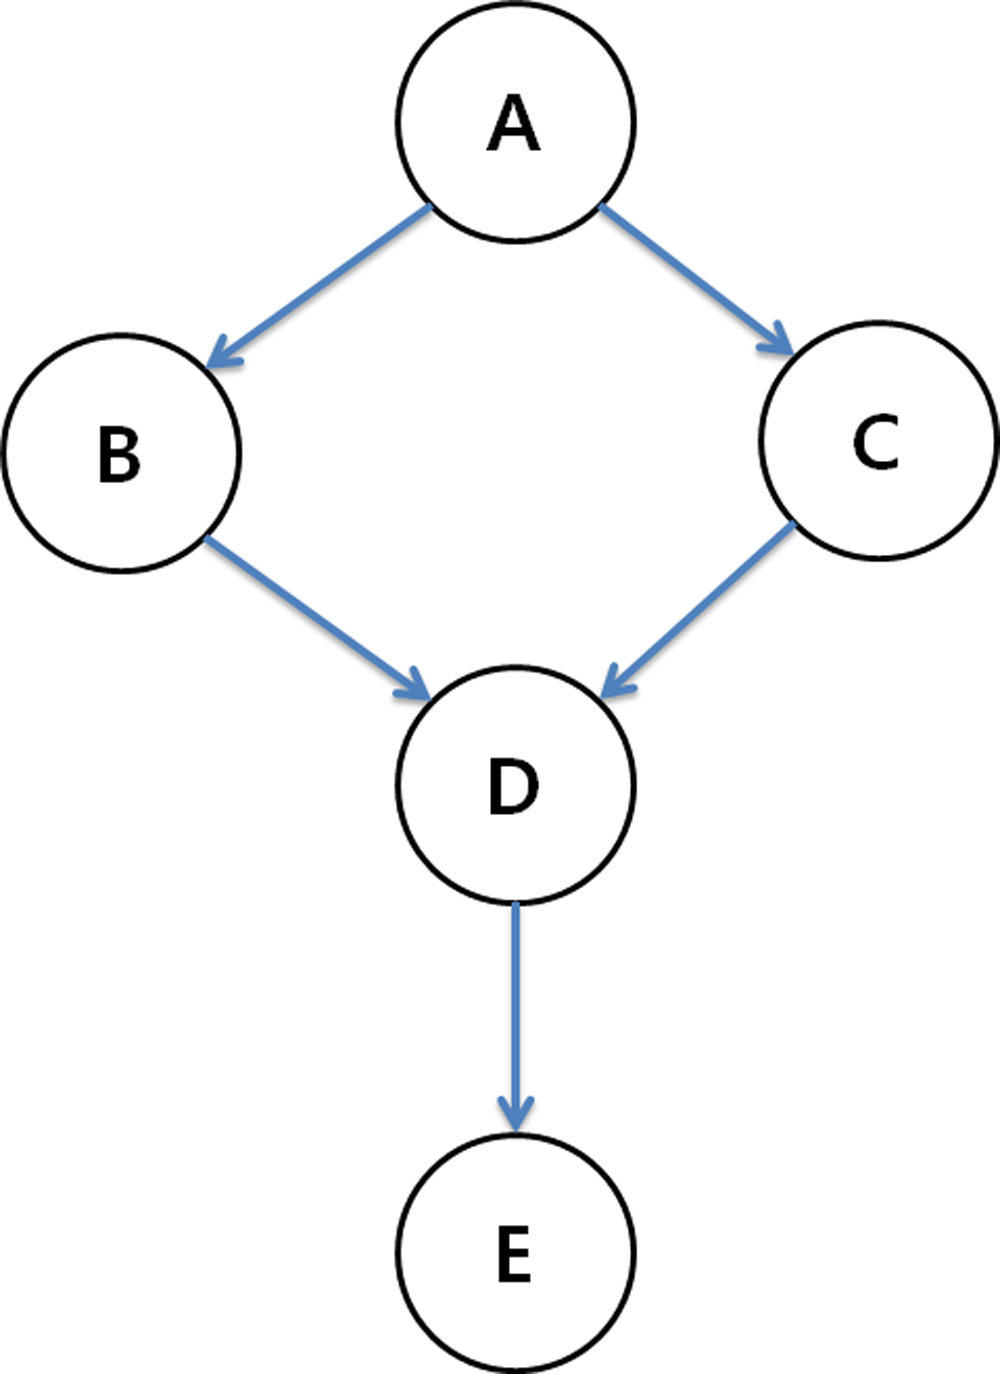
\includegraphics[height=65pt]{images/image01}
		\caption{{\scriptsize{}$P(A,B,C,D,E)=P(A)P(B|A)P(C|A)P(D|B,C)P(E|D)$}}
\end{figure}	
}
\end{frame}

\subsection{Bayesian Network Structure Learning}
\begin{frame}
\frametitle{Bayesian Network Structure Learning}
{\scriptsize{}

Learning a Bayesian network is as follows:

{}\

Given a data $T = \{y_{1}, \cdots, y_{n}\}$ and a scoring function $\phi$, the problem of learning a Bayesian network is to find a Bayesian network $B \in B_{n}$ that maximizes the value $\phi(B, T)$.

{}\

\begin{figure}[!h]
	\centering
		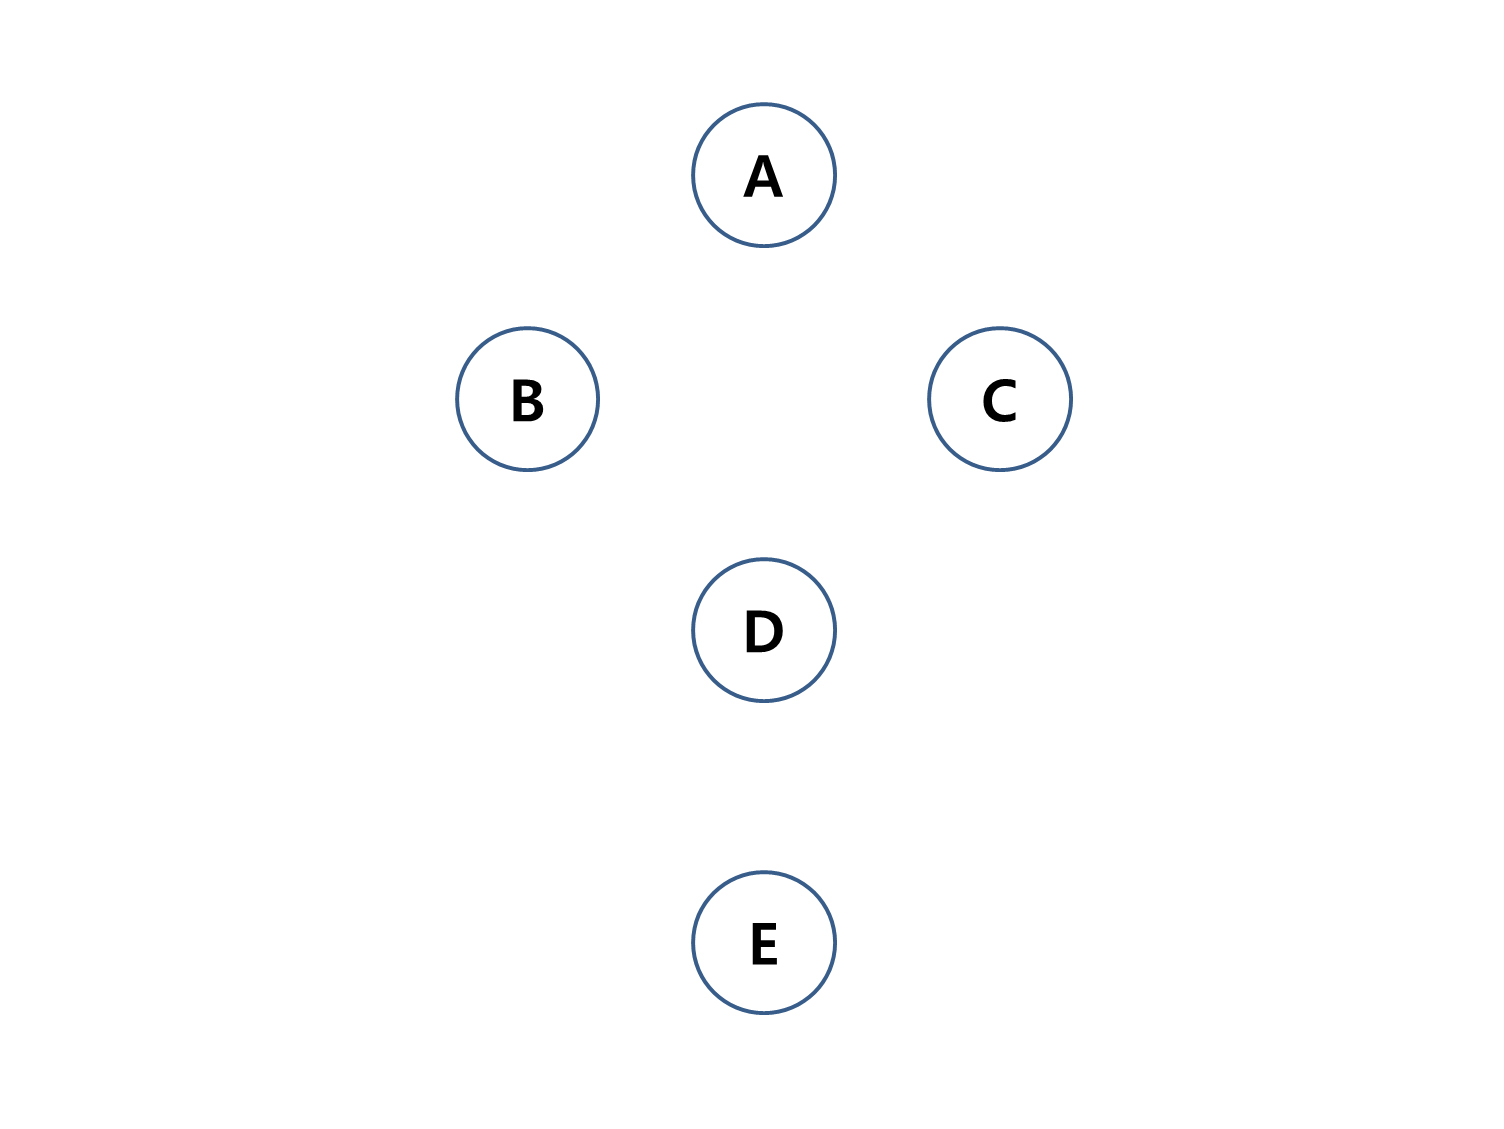
\includegraphics[height=100pt]{images/image02}
		\caption{{\scriptsize{}A model before learning structure}}
\end{figure}	
}
\end{frame}



\section{Structure Learning Algorithms in bnlearn}
\subsection{Available Constraint-based Learning Algorithms}
\begin{frame}
\frametitle{Available Constraint-based learning algorithms}
{\scriptsize{}
\begin{description}
\item[Grow-Shrink (GS)] based on the Grow-Shrink Markov Blanket, the first (and simplest) Markov blanket detection algorithm used in a structure learning algorithm.

{}\

\item[Incremental Association (IAMB)] based on the Markov blanket detection algorithm of the same name, which is based on a two-phase selection scheme (a forward selection followed by an attempt to remove false positives).
\end{description}
}
\end{frame}


\subsection{Available Score-based Learning Algorithms}
\begin{frame}
\frametitle{Available Score-based Learning Algorithms}
{\scriptsize{}
\begin{description}
\item[Hill-Climbing (HC)] a hill climbing greedy search on the space of the directed graphs. The optimized implementation uses score caching, score decomposability and score equivalence to reduce the number of duplicated tests.

{}\

\item[Tabu Search (TABU)] a modified hill climbing able to escape local optima by selecting a network that minimally decreases the score function.
\end{description}
}
\end{frame}


\subsection{Available Hybrid Learning Algorithms}
\begin{frame}
\frametitle{Available Hybrid Learning Algorithms}
{\scriptsize{}
\begin{description}
\item[Max-Min Hill-Climbing (MHHC)] a hybrid algorithm which combines the Max-Min Parents and Children algorithm (to restrict the search space) and the Hill-Climbing algorithm (to find the optimal network structure in the restricted space).

{}\

\item[Restricted Maximization (RSMAX2)] a more general implementation of the Max-Min Hill-Climbing, which can use any combination of constraint-based and score-based algorithms.
\end{description}
}
\end{frame}



\section{The Comparison Methodology}
\subsection{The Number of Graphical Errors in the Learnt Structure}
\begin{frame}
\frametitle{The Number of Graphical Errors in the Learnt Structure}
{\scriptsize{}

In terms of the number of graphical errors in the learnt structure.

{}\
	
\begin{center}
\begin{tabular}{c|l|c|c|c}
\hline 
& & \textbf{Target Network} & \textbf{Learnt Network} & \textbf{Direction}\tabularnewline
\hline 
\textbf{\textcolor{blue}{C}} & (Correct Arcs) & exist & exist & correct\tabularnewline
\textbf{\textcolor{blue}{M}} & (Missing Arcs) & exist & \textcolor{red}{not exist} & \tabularnewline
\textbf{\textcolor{blue}{WO}} & (Wrongly Oriented Arcs) & exist & exist & \textcolor{red}{wrong}\tabularnewline
\textbf{\textcolor{blue}{WC}} & (Wrongly Corrected Arcs) & not exist & \textcolor{red}{exist} & \tabularnewline
\hline 
\end{tabular}
\end{center}
}
\end{frame}




	
\subsection{Network Scores}
\begin{frame}
\frametitle{Network Scores}
{\scriptsize{}
In all four cases, the higher the value of the metric, the better the network.
\begin{description}
	\item[BDe]
	$BDe(B,T) = P(B,T)=P(B)\times\prod_{i=1}^{n}\prod_{j=1}^{q_{i}}(\frac{\Gamma(N'_{ij})}{\Gamma(N_{ij}+N'_{ij})}\times\prod_{k=1}^{r_{i}}\frac{\Gamma(N_{ijk}+N'_{ijk})}{\Gamma(N'_{ijk})})$
\end{description}

{}\

$$\phi(B|T) = LL(B|T) - f(N)|B|,$$

\begin{description}
	\item[Log-Likelihood(LL)] If $f(N) = 0$, we have the \textbf{LL} score.
	
	\item[AIC] If f(N) = 1, we have the \textbf{AIC} scoring function:
	
	\item[BIC] If $f(N) = \frac{1}{2} \log(N)$, we have the \textbf{BIC} score.
\end{description}
}
\end{frame}






\section{Data Generation with BN$\_$Data$\_$Generator in R}

\begin{frame}
\frametitle{Data Generation with BN$\_$Data$\_$Generator in R}

{\scriptsize{}
	\textbf{BN$\_$Data$\_$Generator} $\{$User-Defined Function$\}$

	{}\	
	
	\begin{description}
		\item[Description] It based on a Bayesian network model to generates synthetic data.
		
		{}\
		
		\item[Usage] BN$\_$Data$\_$Generator (arcs, input$\_$Probs, n, node$\_$names)

		{}\
		
		\item[URL] https://github.com/praster1/BN$\_$Data$\_$Generator		

		{}\
		
		\item[Arguments]
	\end{description}
	
	\begin{center}
				\begin{tabular}{c|c|l}
					\hline 
					\textbf{arcs} & (matrix) & A matrix that determines the arcs.\tabularnewline
					\hline 
					\textbf{input$\_$Probs} & (list) & The conditional probabilities.\tabularnewline
					\hline 
					\textbf{n} & (constant) & Sample Size\tabularnewline
					\hline 
					\textbf{node$\_$names} & (vector) & Node names\tabularnewline
					\hline 
				\end{tabular}
	\end{center}
}
\end{frame}




\begin{frame}
\frametitle{Data Generation with BN$\_$Data$\_$Generator in R}

{\scriptsize{}
	\begin{center}
		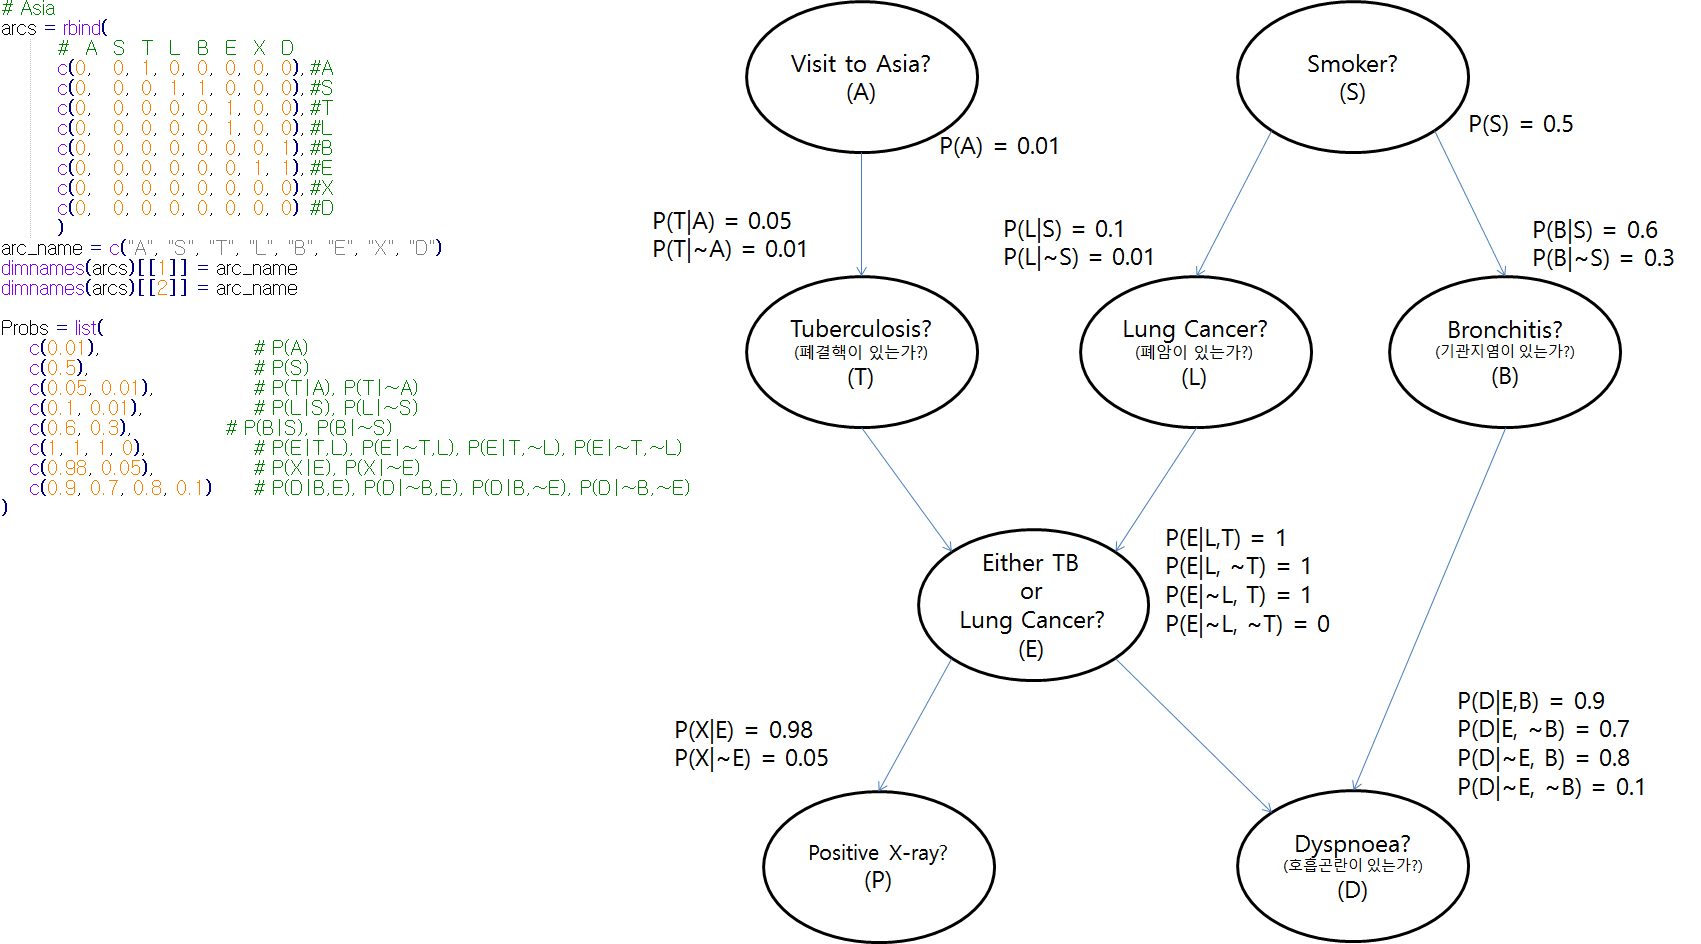
\includegraphics[height=170pt]{images/image24}
	\end{center}
}
\end{frame}



\begin{frame}
\frametitle{Data Generation with BN$\_$Data$\_$Generator in R}
{\scriptsize{}
	\begin{center}
		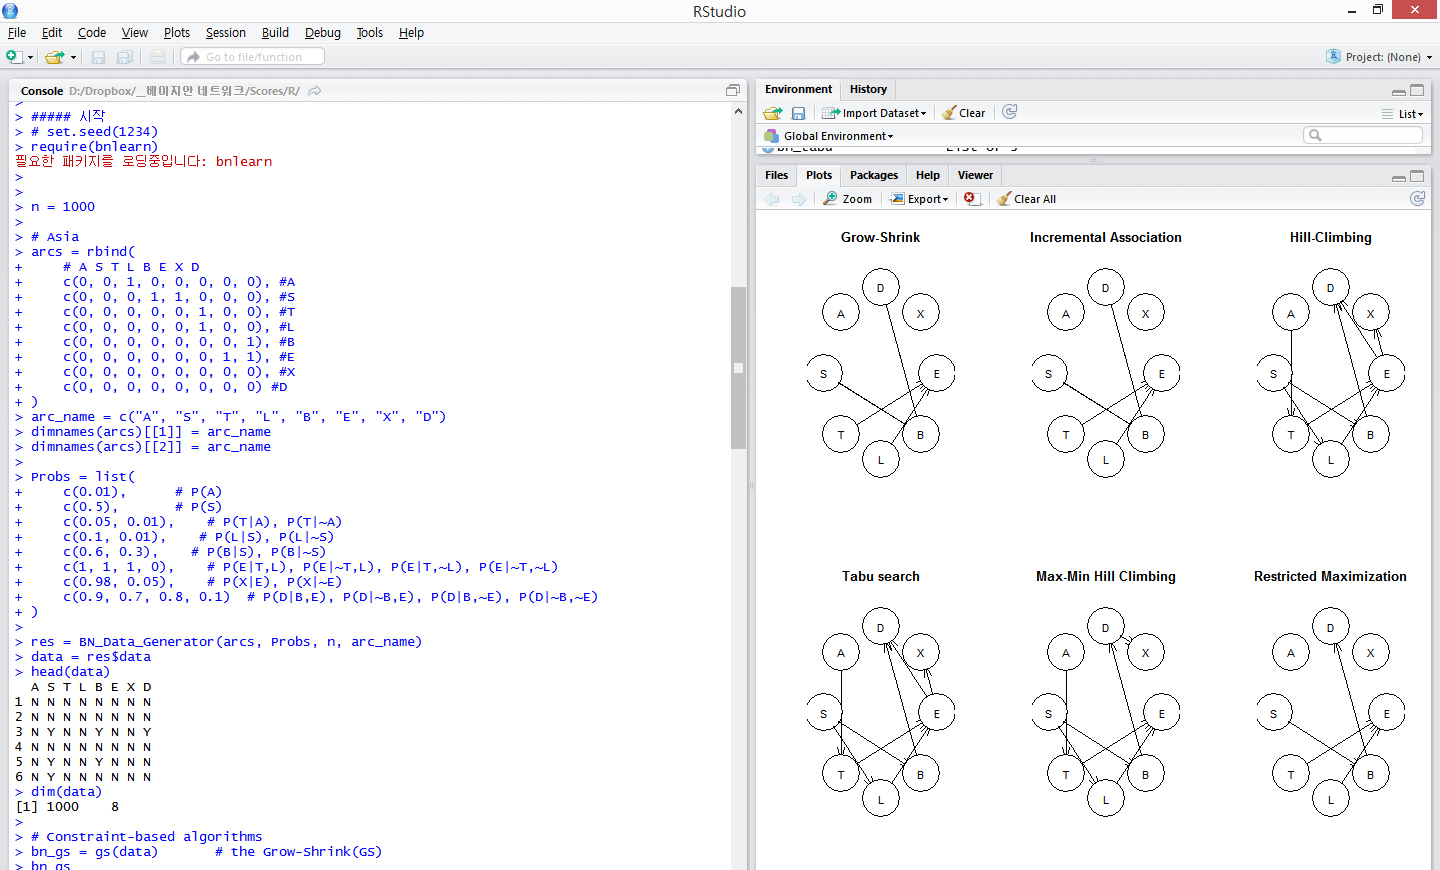
\includegraphics[height=170pt]{images/image23}
	\end{center}
}
\end{frame}


\section{Simulation}

\begin{frame}
\frametitle{Outline}
{\scriptsize{}
	\tableofcontents[currentsection]
}
\end{frame}


\subsection{Real Datasets}



\begin{frame}
\frametitle{Prerequisite}
{\scriptsize{}
	\begin{itemize}
		\item All experiments are \textcolor{red}{repeated 100 times}, and overall results are reported.
		
		{}\		
		
		\item \textcolor{red}{Constraint-based} Learning Algorithms often makes \textcolor{red}{undirected arcs}. So, this has been excluded from comparison.
		
	\end{itemize}
}
\end{frame}


\begin{frame}
\frametitle{Asia DataSet}
{\scriptsize{}
\begin{description}
	\item[Description] Small synthetic data set from Lauritzen and Spiegelhalter (1988) about lung diseases (tuberculosis, lung cancer or bronchitis) and visits to Asia.
	
	\item[Number of nodes] 8
	
	\item[Number of arcs] 8
	
	\item[Number of parameters] 18
	
	\item[Source] Lauritzen S, Spiegelhalter D (1988).
	
	"Local Computation with Probabilities on Graphical Structures and their Application to Expert Systems (with discussion)".
	
	Journal of the Royal Statistical Society: Series B (Statistical Methodology), 50(2), 157-224.
\end{description}
}
\end{frame}


\begin{frame}
\frametitle{Asia DataSet}
{\scriptsize{}
	\begin{figure}
		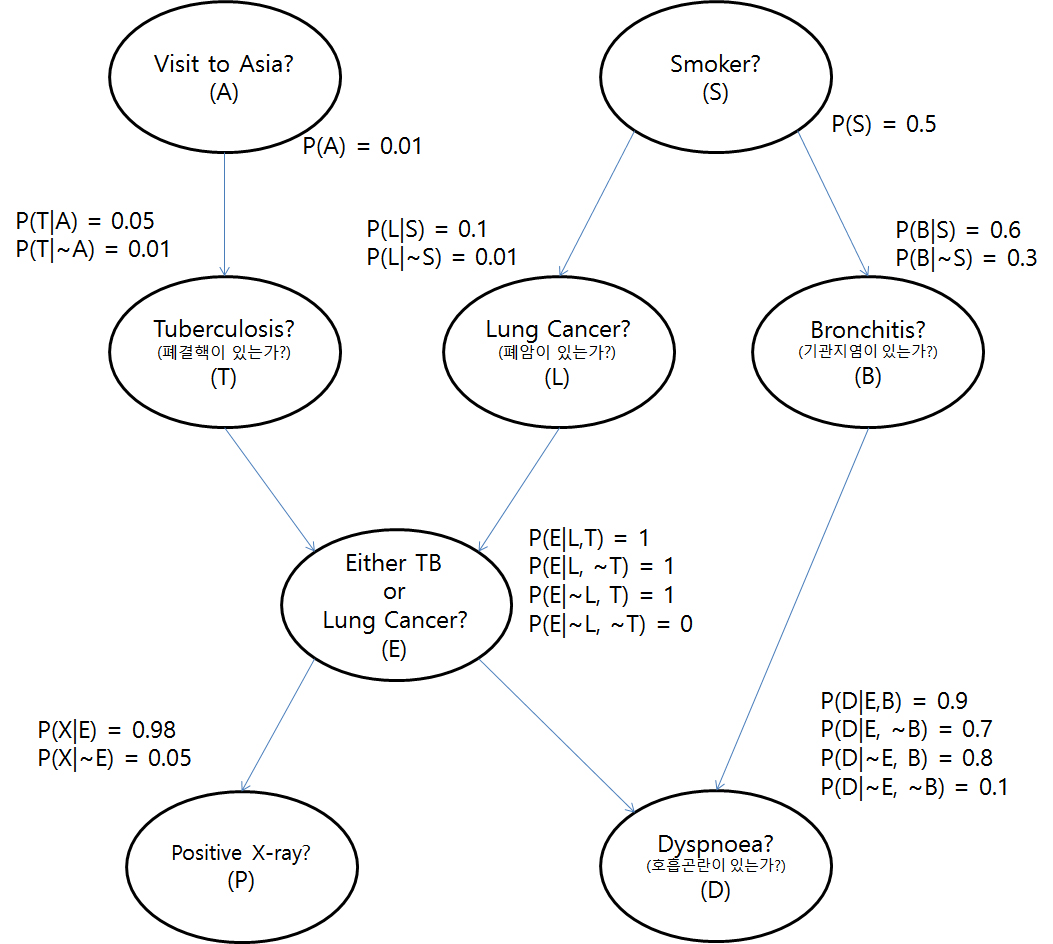
\includegraphics[height=170pt]{images/Model_Real_Asia}
	\end{figure}	
}
\end{frame}



\begin{frame}
\frametitle{Insurance DataSet}
{\scriptsize{}
\begin{description}
	\item[Description] Insurance is a network for evaluating car insurance risks.
	
	\item[Number of nodes] 27
	
	\item[Number of arcs] 52
	
	\item[Number of parameters] 984
	
	\item[Source]  Binder J, Koller D, Russell S, Kanazawa K (1997).

	 "Adaptive Probabilistic Networks with Hidden Variables".
	 
	  Machine Learning, 29(2-3), 213-244.
\end{description}
}
\end{frame}



\begin{frame}
\frametitle{Insurance DataSet}
{\scriptsize{}
	\begin{figure}
		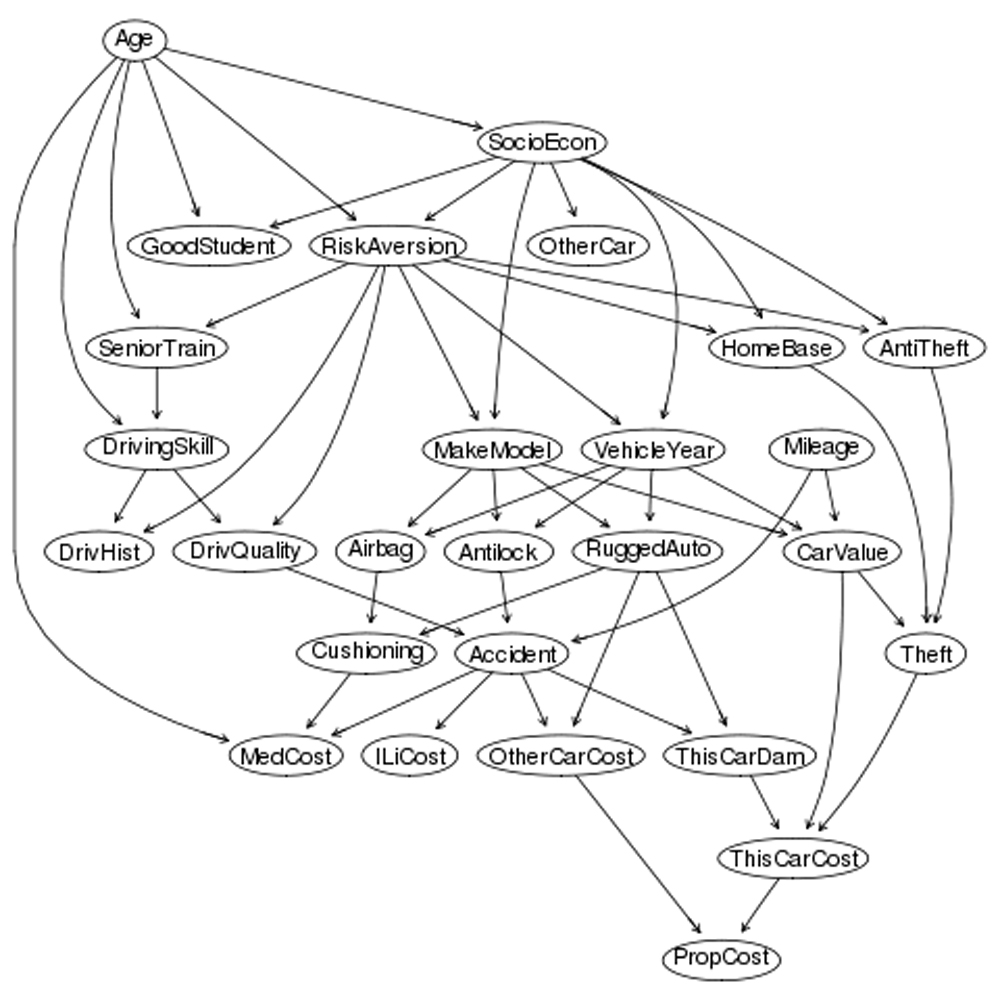
\includegraphics[height=170pt]{images/Model_Real_Insurance}
	\end{figure}	
}
\end{frame}



\begin{frame}
\frametitle{Alarm DataSet}
{\scriptsize{}
\begin{description}
	\item[Description] The ALARM ("A Logical Alarm Reduction Mechanism") is a Bayesian network designed to provide an alarm message system for patient monitoring.
	
	\item[Number of nodes] 37
	
	\item[Number of arcs] 46
	
	\item[Number of parameters] 509
	
	\item[Source]  Beinlich I, Suermondt HJ, Chavez RM, Cooper GF (1989).
	
	"The ALARM Monitoring System: A Case Study with Two Probabilistic Inference Techniques for Belief Networks."
	
	In "Proceedings of the 2nd European Conference on Artificial Intelligence in Medicine", pp. 247-256. Springer-Verlag.
\end{description}
}
\end{frame}


\begin{frame}
\frametitle{Alarm DataSet}
{\scriptsize{}
	\begin{figure}
		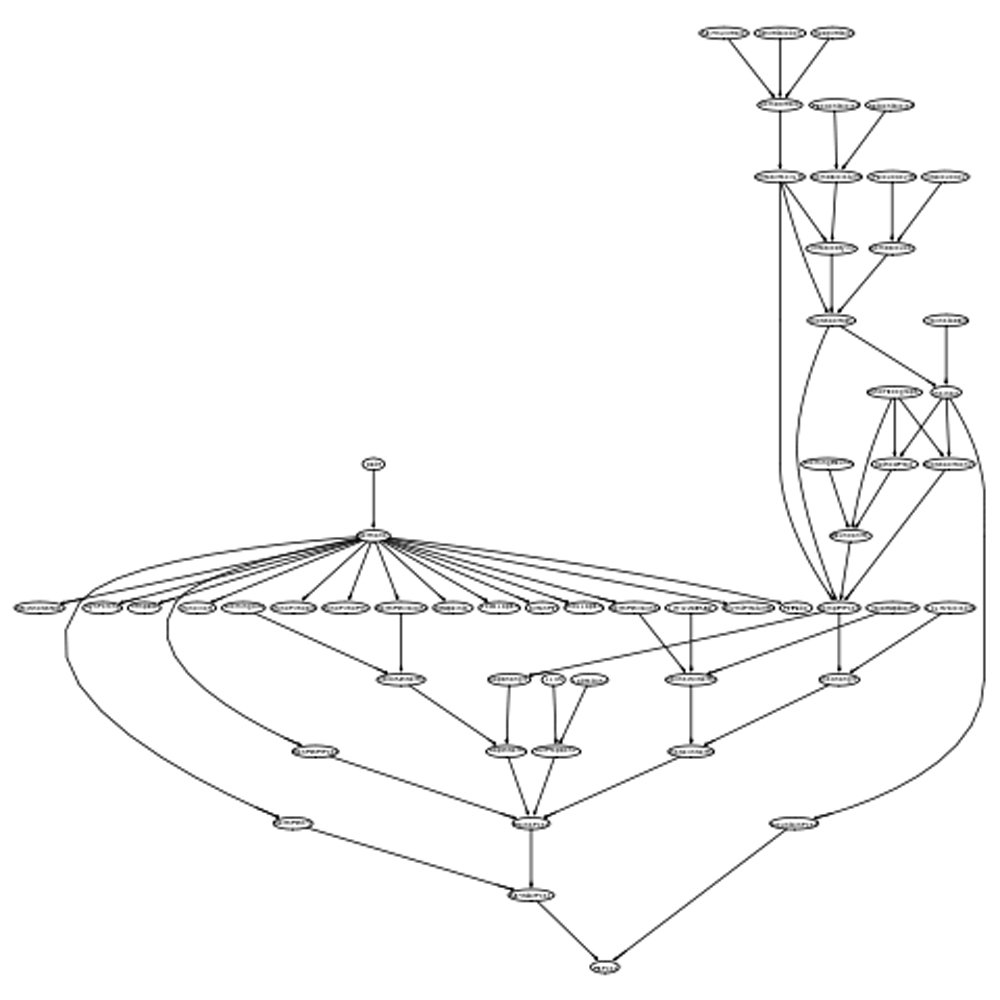
\includegraphics[height=170pt]{images/Model_Real_ALARM}
	\end{figure}	
}
\end{frame}



\begin{frame}
\frametitle{HailFinder DataSet}
{\scriptsize{}
\begin{description}
	\item[Description] Hailfinder is a Bayesian network designed to forecast severe summer hail in northeastern Colorado.
	
	\item[Number of nodes] 56
	
	\item[Number of arcs] 66
	
	\item[Number of parameters] 2656
	
	\item[Source]  Abramson B, Brown J, Edwards W, Murphy A, Winkler RL (1996).
	
	"Hailfinder: A Bayesian system for forecasting severe weather".
	
	International Journal of Forecasting, 12(1), 57-71.
\end{description}
}
\end{frame}


\begin{frame}
\frametitle{HailFinder DataSet}
{\scriptsize{}
	\begin{figure}
		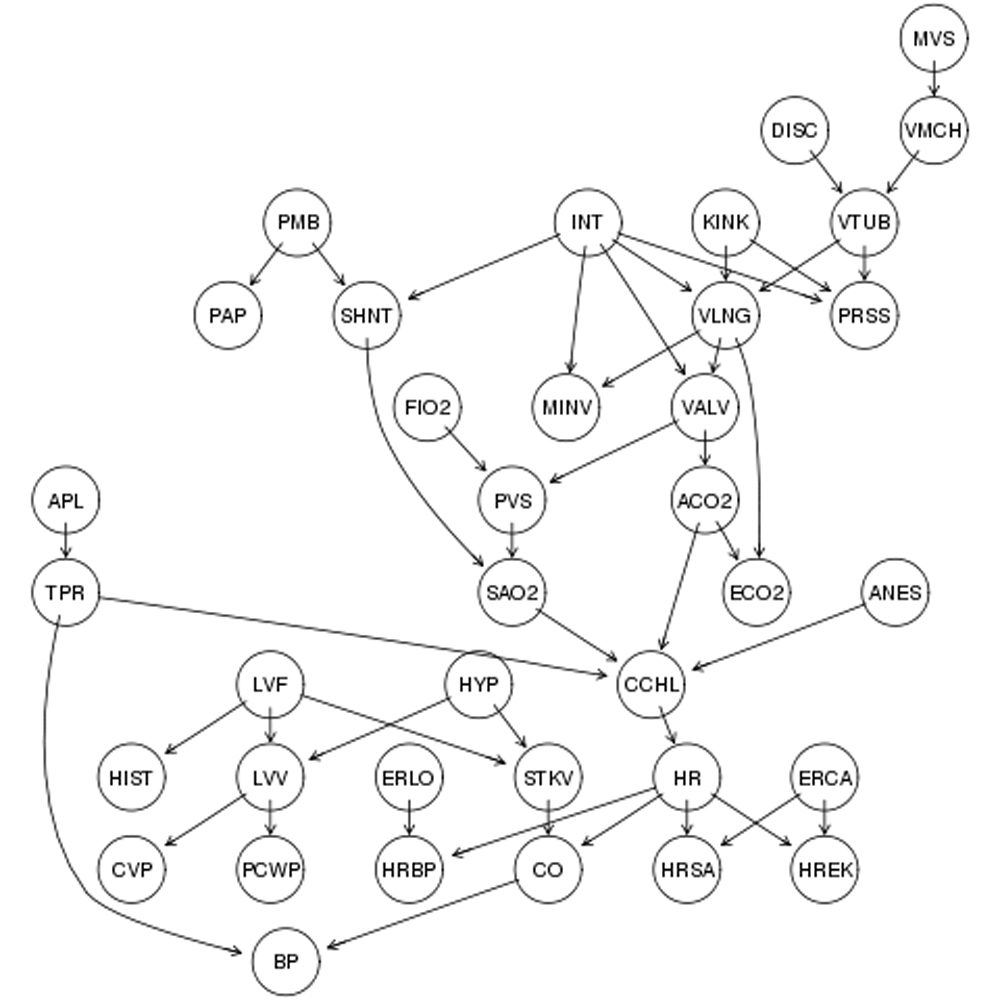
\includegraphics[height=170pt]{images/Model_Real_Hailfinder}
	\end{figure}	
}
\end{frame}



\begin{frame}
\frametitle{Summary}
{\scriptsize{}
	\begin{center}
		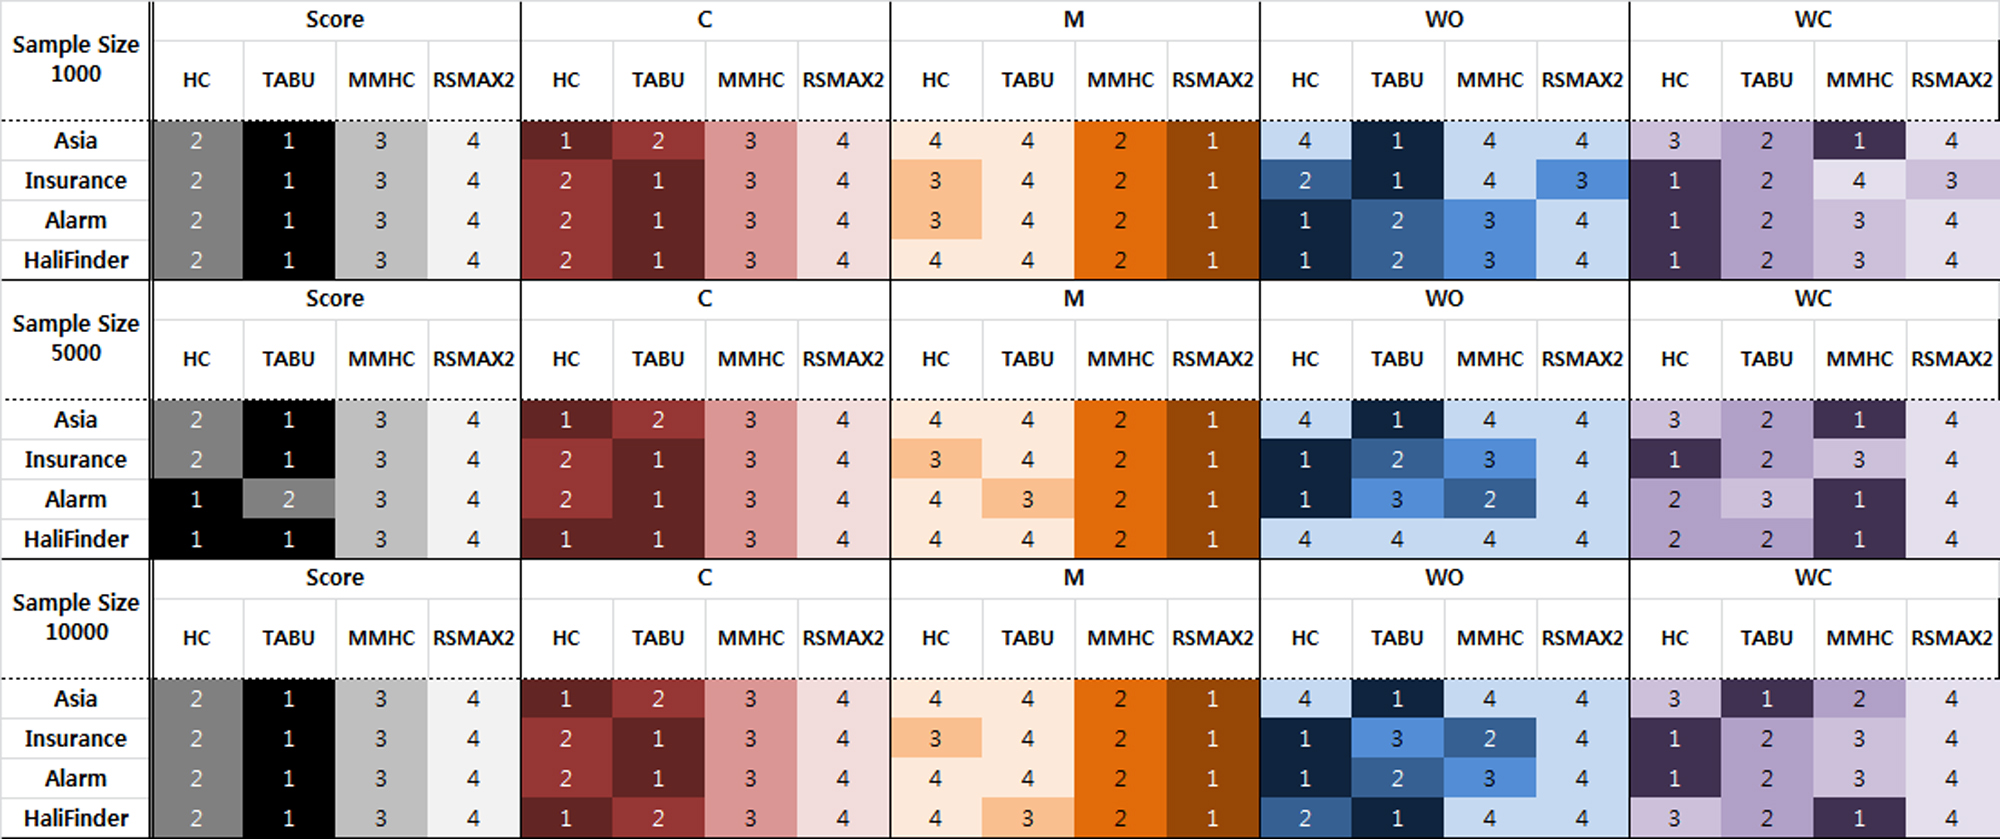
\includegraphics[height=130pt]{images/Real_Result}
	\end{center}
}
\end{frame}


\subsection{Synthetic Data According to Topologies}
\begin{frame}
\frametitle{Varying topologies and number of nodes}
{\scriptsize{}
	\begin{center}
		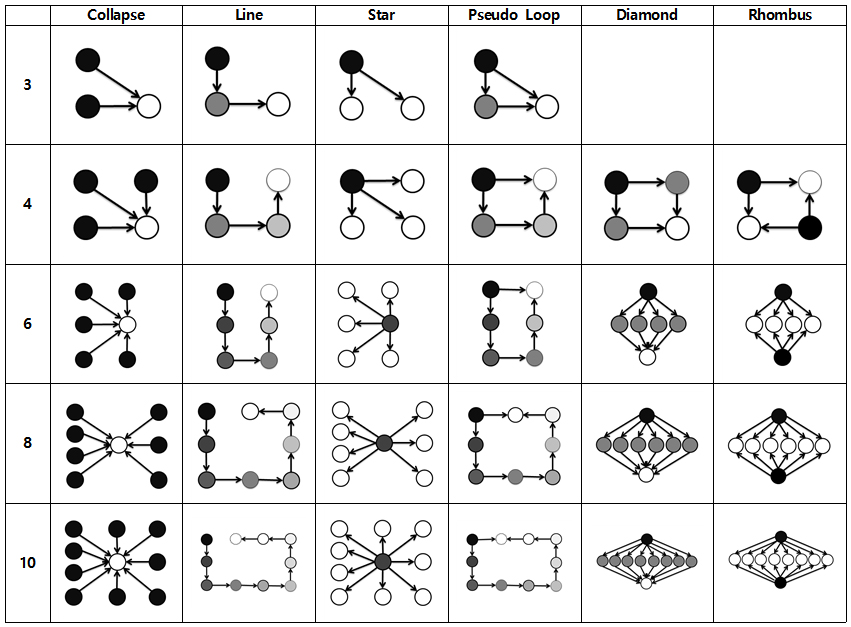
\includegraphics[height=150pt]{images/image21}
	\end{center}		
}
\tiny{
		Eitel J. M. Lauría,
		
		"An Information-Geometric Approach to Learning Bayesian Network Topologies from Data",
		
		Innovations in Bayesian Networks Studies in Computational Intelligence Volume 156, 2008, pp 187-217
		}
\end{frame}


\begin{frame}
\frametitle{Prerequisite}
{\scriptsize{}
	\begin{itemize}
		\item \textcolor{red}{Cardinality} was limited to \textcolor{red}{two}.

		{}\

		\item \textcolor{red}{The probability value}, which is imparted optionally under \textcolor{red}{U(0, 1)} distribution.

		{}\

		\item All experiments are \textcolor{red}{repeated 100 times}, and overall results are reported.
		
		{}\		
		
		\item \textcolor{red}{Constraint-based} Learning Algorithms often makes \textcolor{red}{undirected arcs}. So, this has been excluded from comparison.
		
	\end{itemize}
}
\end{frame}


\begin{frame}
\frametitle{Collapse}
{\scriptsize{}
	\begin{figure}
		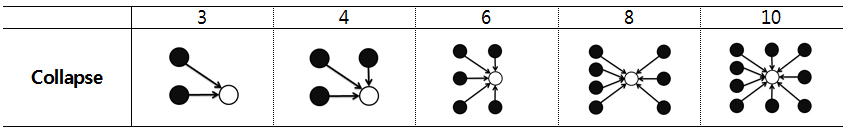
\includegraphics[height=50pt]{images/Topologies_Collapse}
	\end{figure}	
}
\end{frame}



\begin{frame}
\frametitle{Collapse (Score)}
{\scriptsize{}
	\begin{figure}
		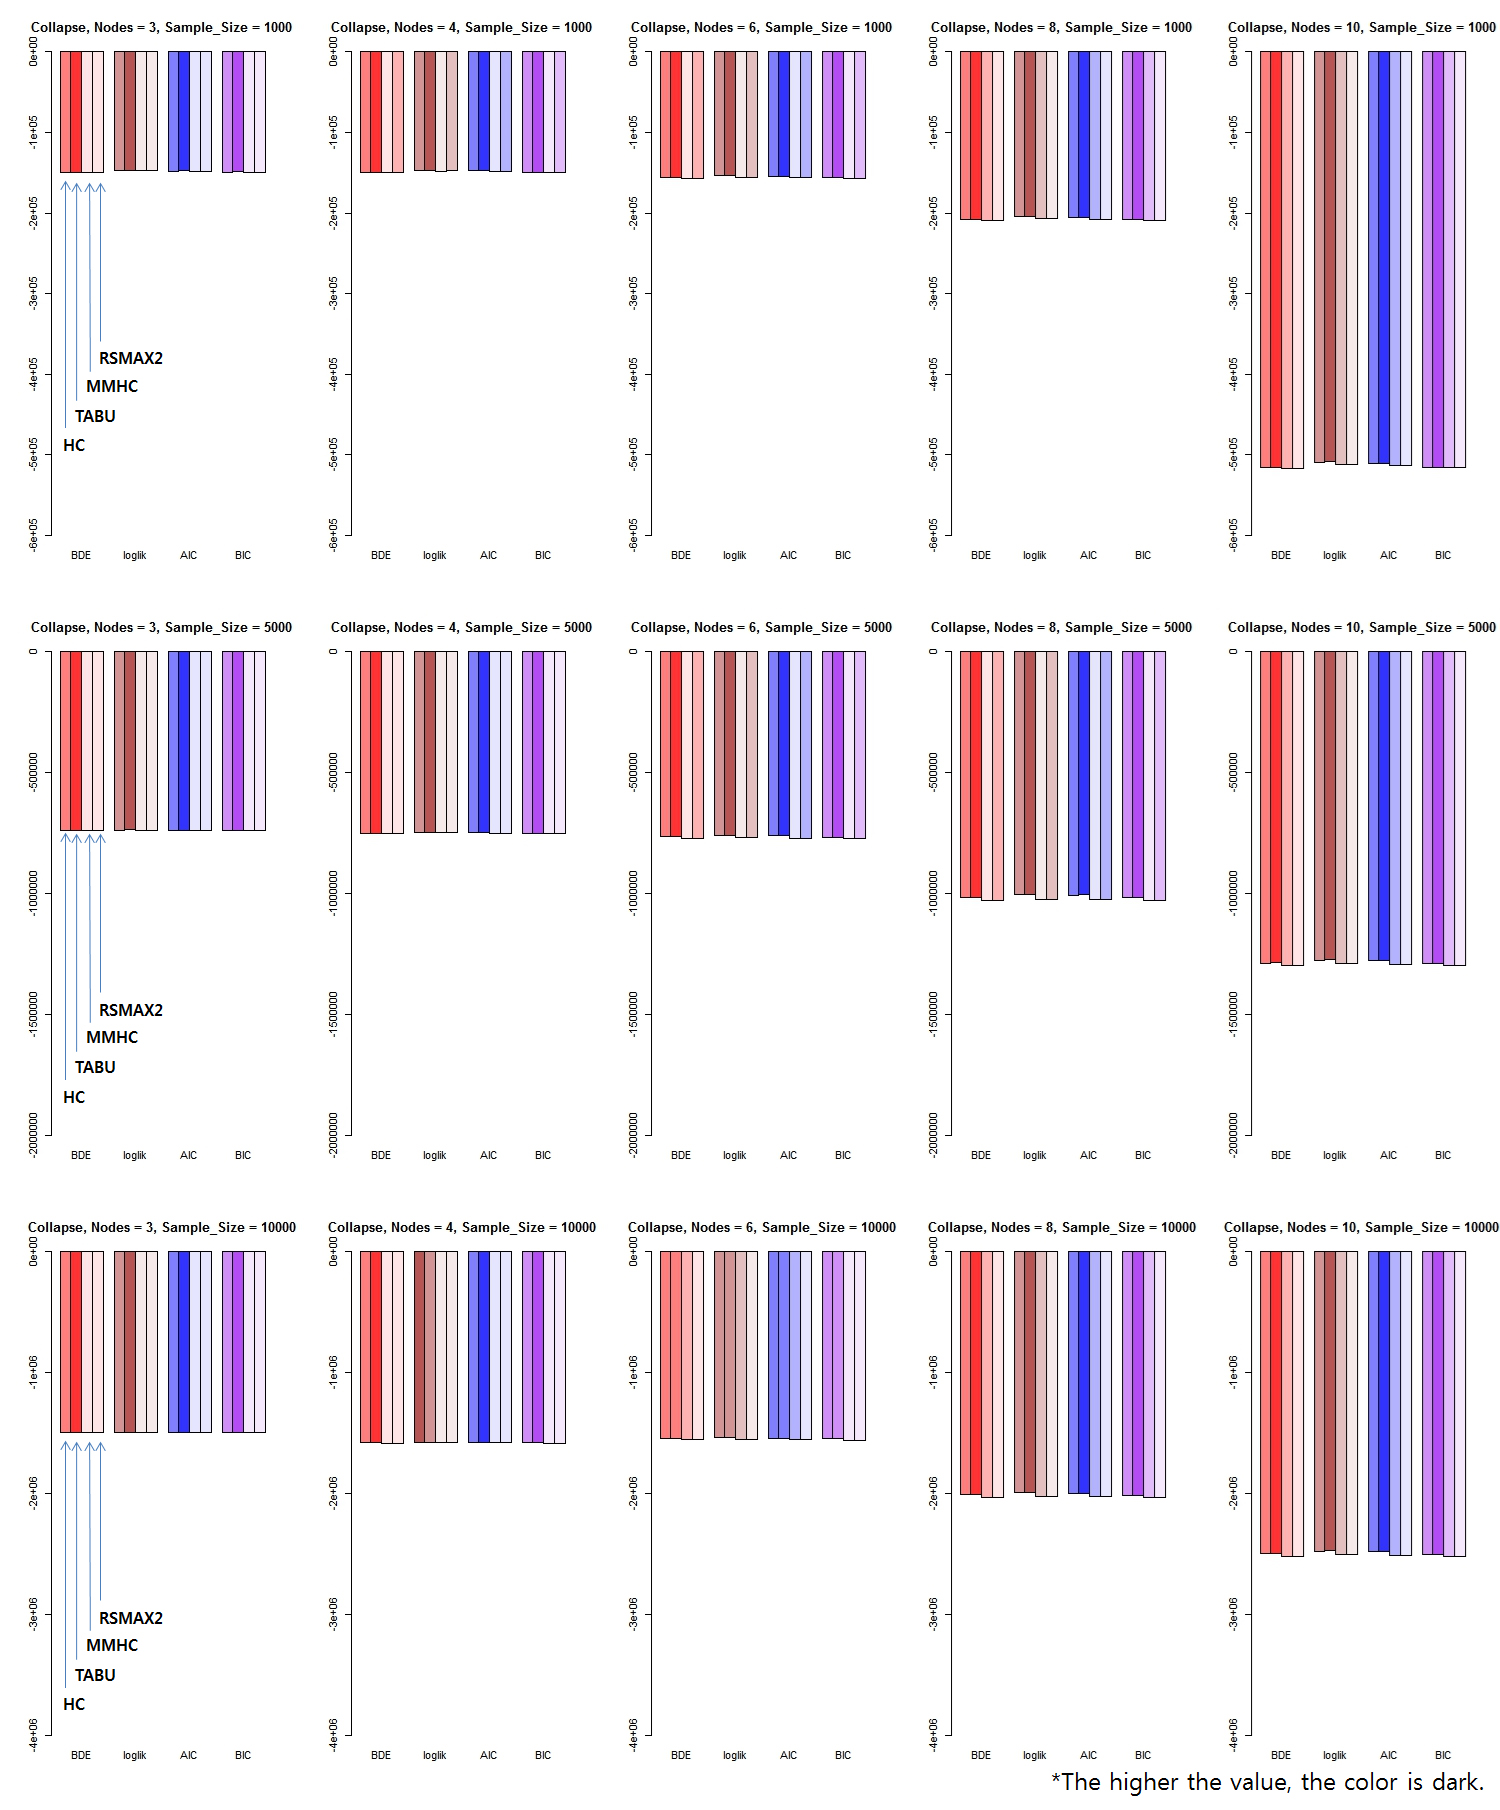
\includegraphics[height=170pt]{images/01_Collapse_Score}
	\end{figure}	
}
\end{frame}


\begin{frame}
\frametitle{Collapse (Arcs)}
{\scriptsize{}
	\begin{figure}
		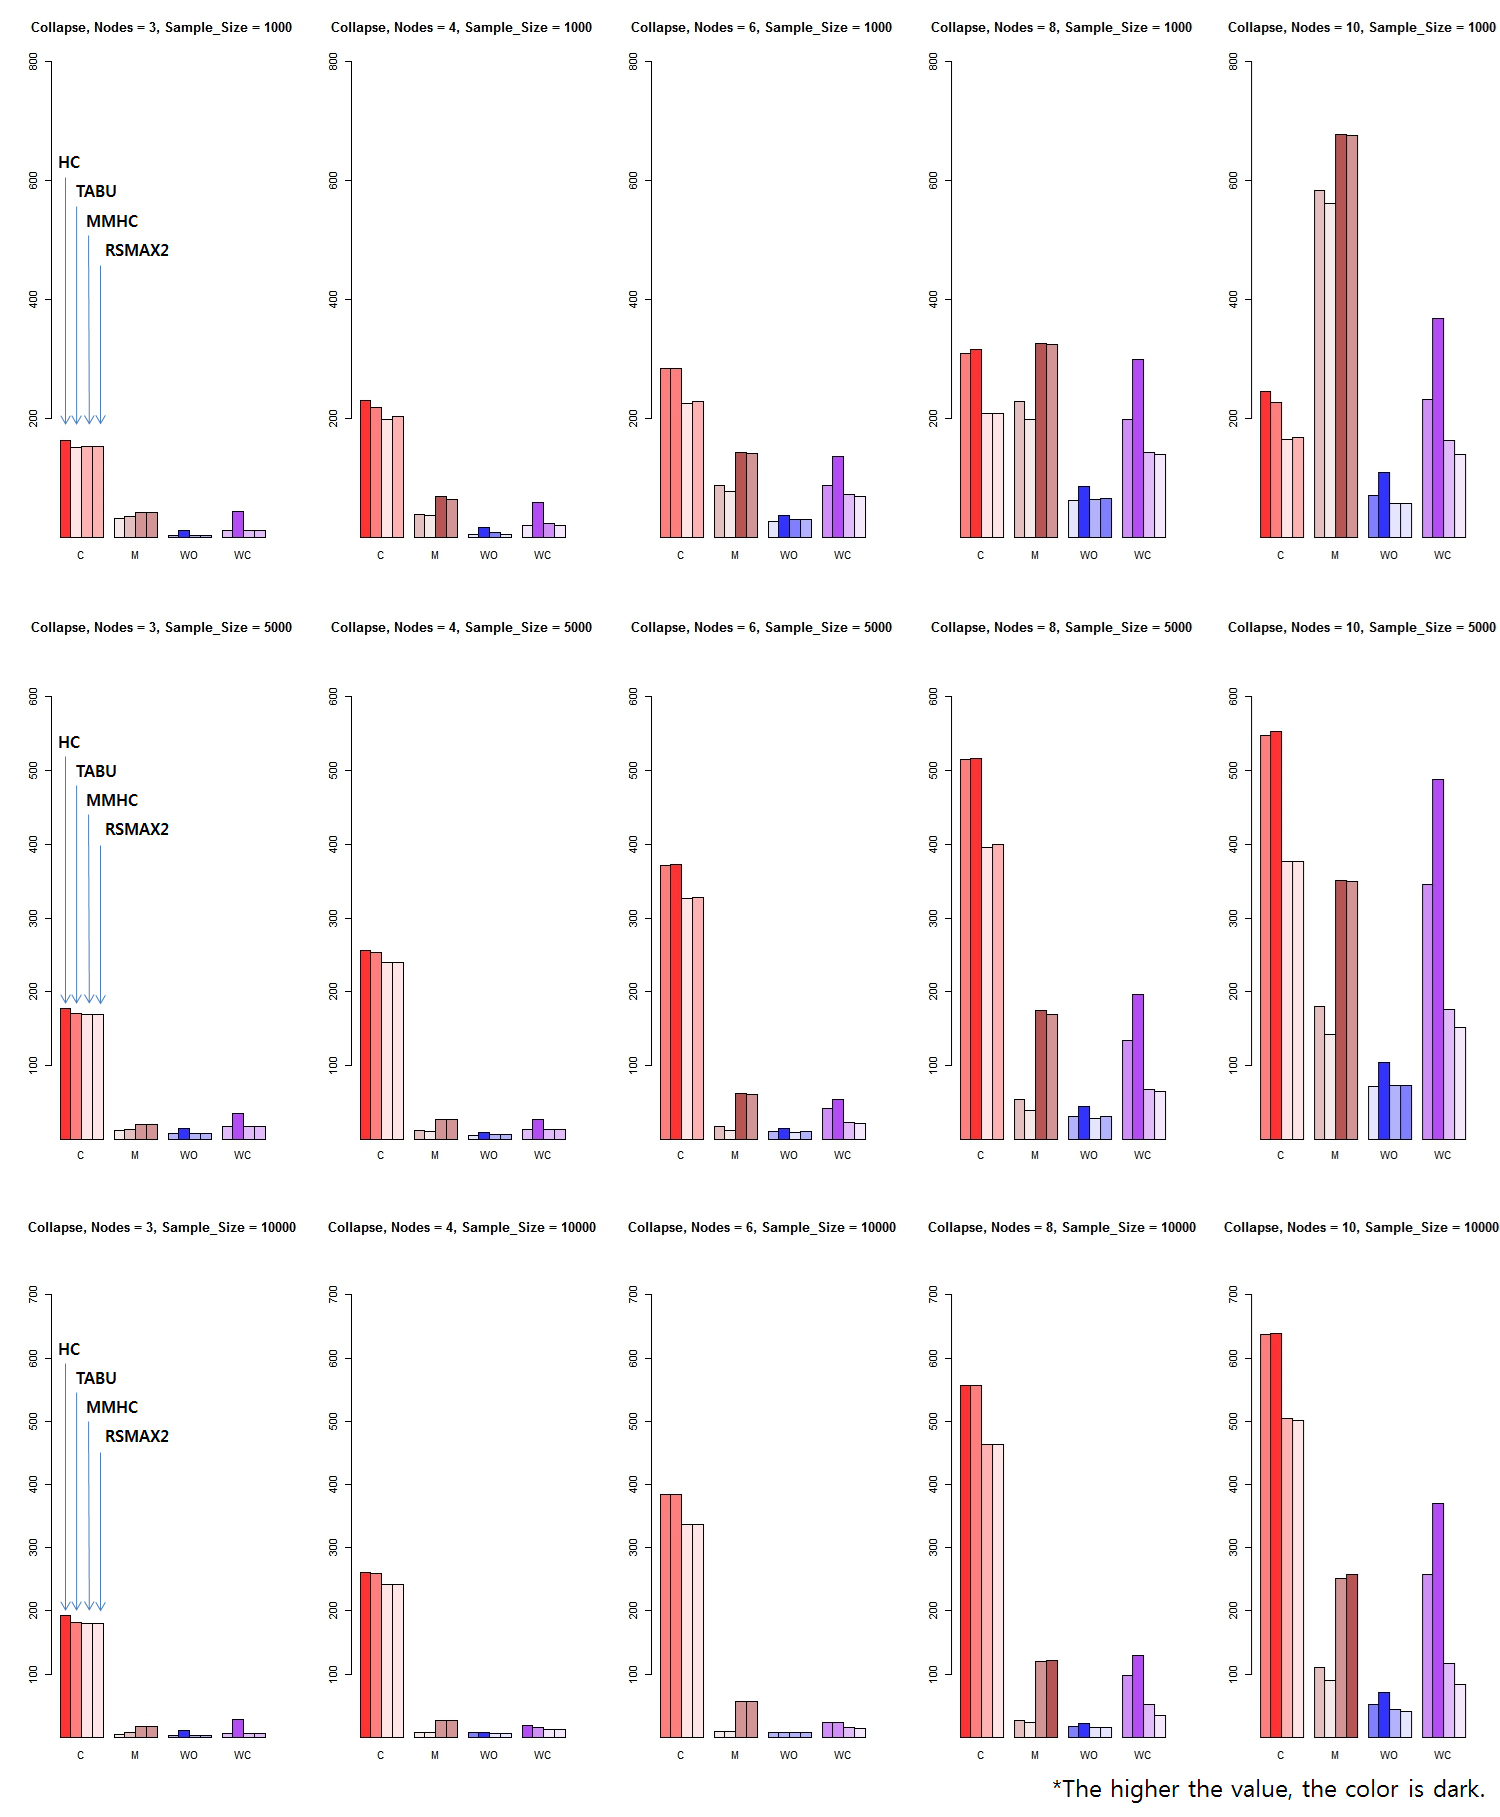
\includegraphics[height=170pt]{images/01_Collapse_Arcs}
	\end{figure}	
}
\end{frame}



\begin{frame}
\frametitle{Collapse}
{\scriptsize{}
	\begin{center}
		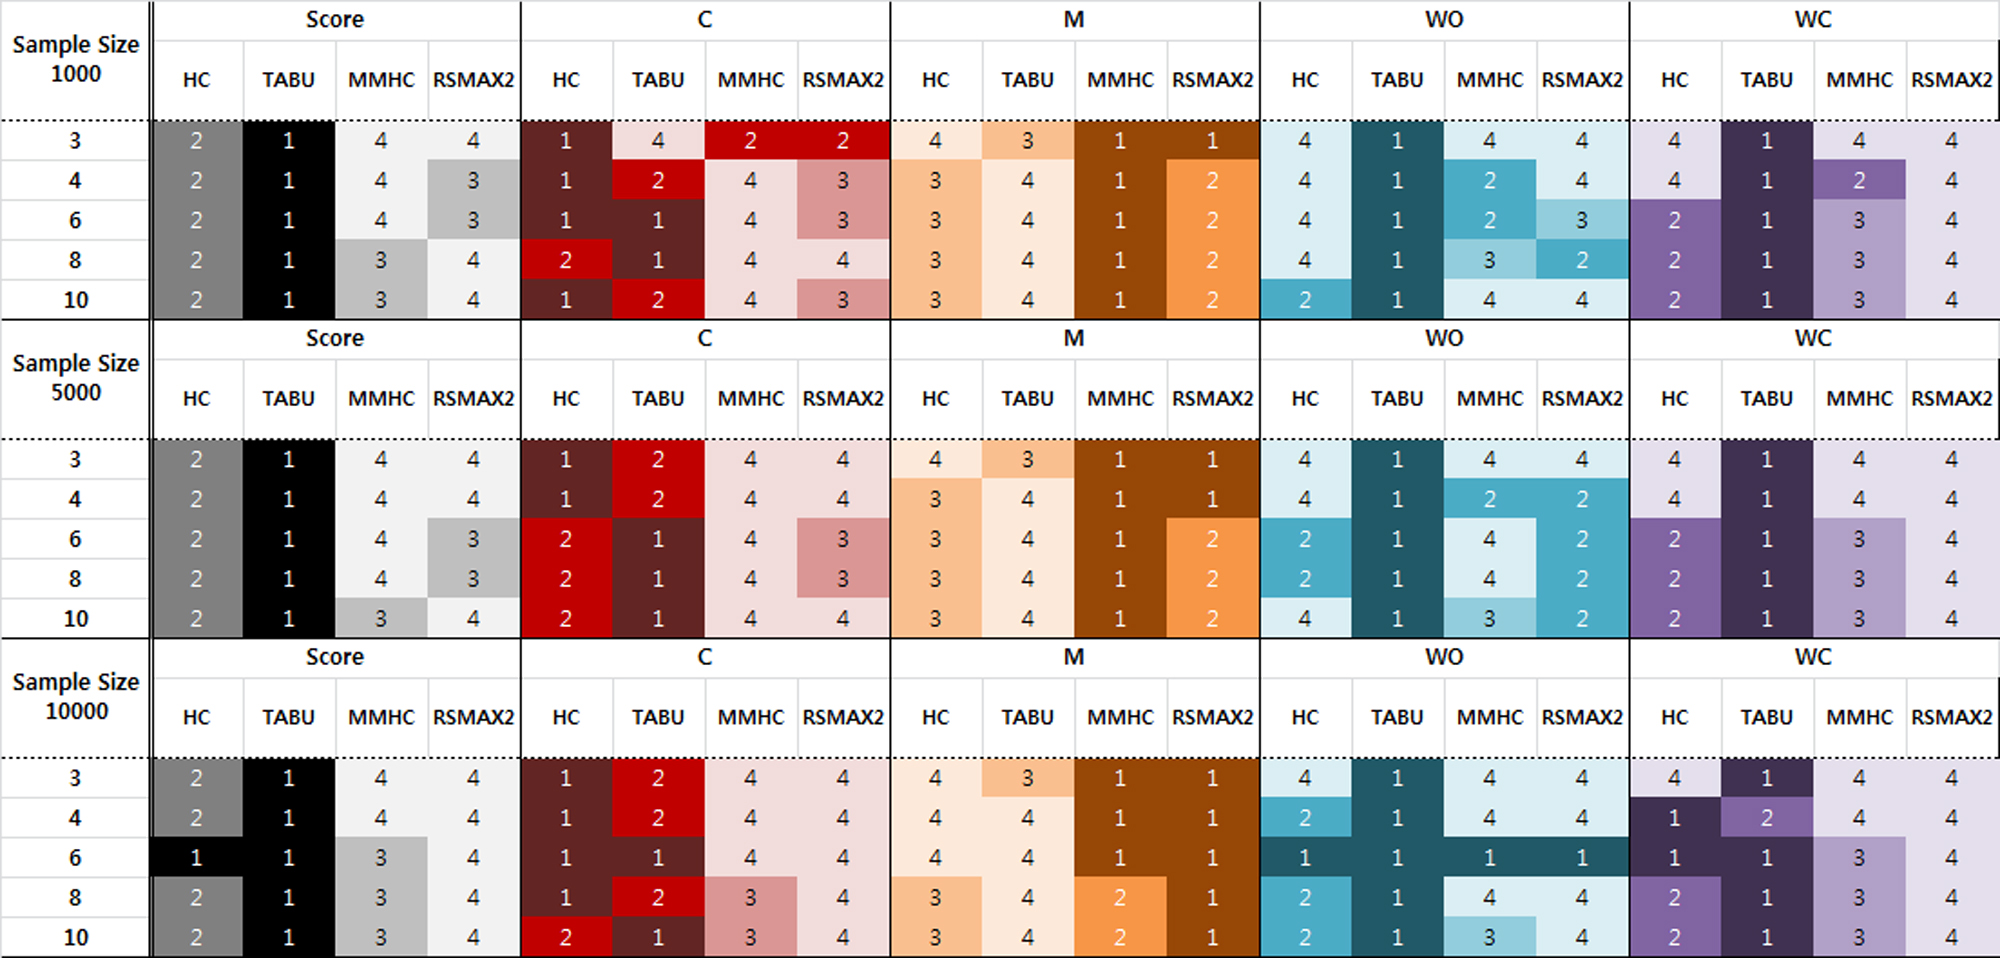
\includegraphics[height=130pt]{images/Result_Collapse}
	\end{center}
}
\end{frame}



\begin{frame}
\frametitle{Line}
{\scriptsize{}
	\begin{figure}
		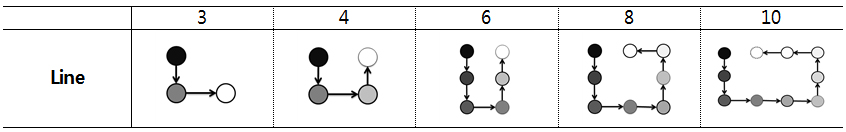
\includegraphics[height=50pt]{images/Topologies_Line}
	\end{figure}	
}
\end{frame}



\begin{frame}
\frametitle{Line (Score)}
{\scriptsize{}
	\begin{figure}
		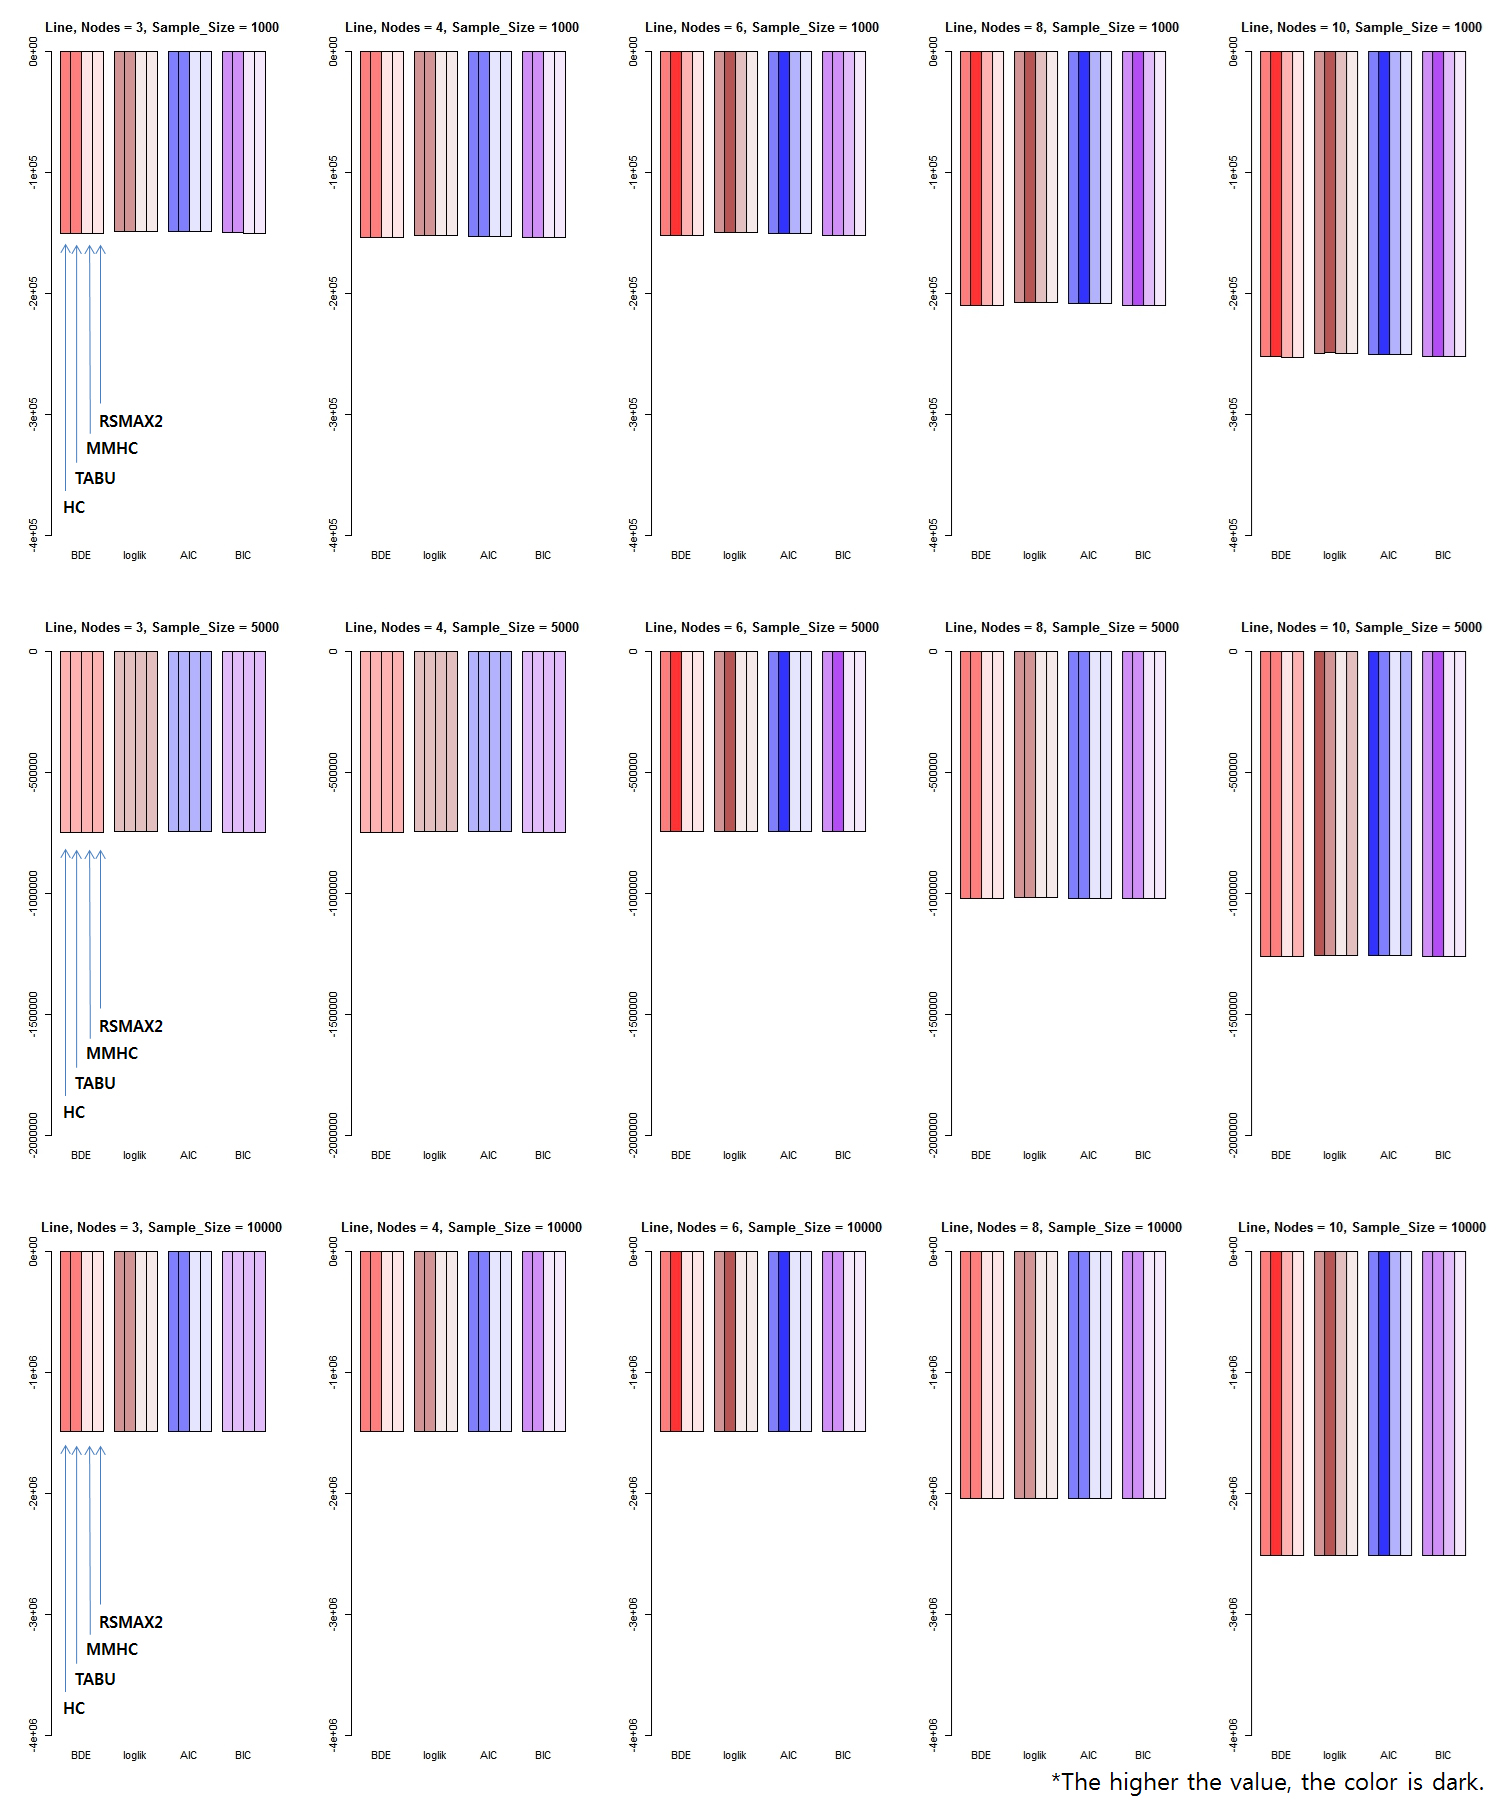
\includegraphics[height=170pt]{images/02_Line_Score}
	\end{figure}	
}
\end{frame}


\begin{frame}
\frametitle{Line (Arcs)}
{\scriptsize{}
	\begin{figure}
		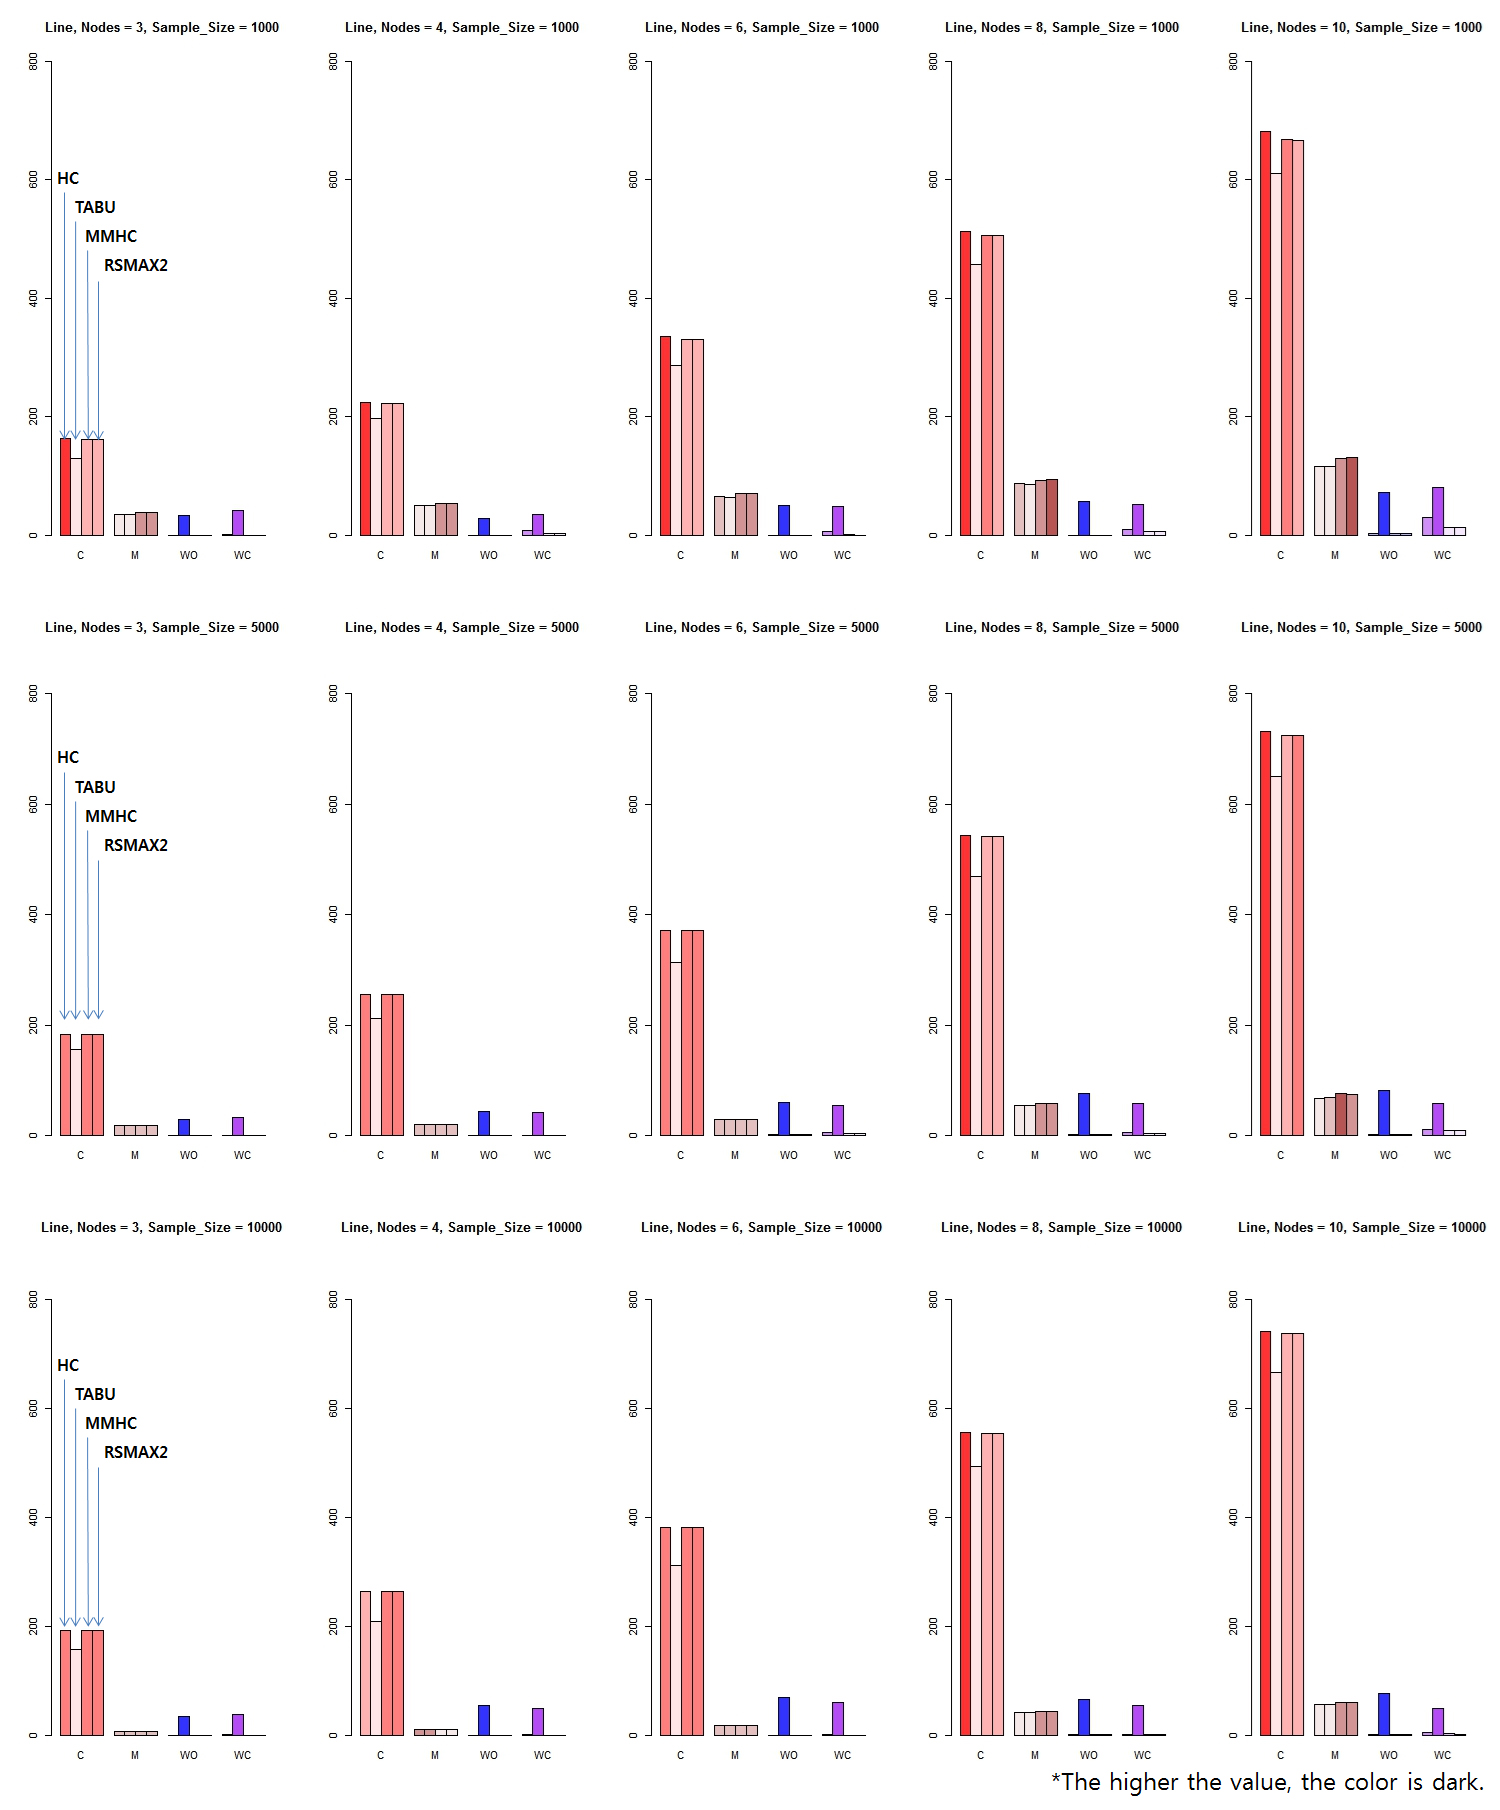
\includegraphics[height=170pt]{images/02_Line_Arcs}
	\end{figure}	
}
\end{frame}



\begin{frame}
\frametitle{Line}
{\scriptsize{}
	\begin{center}
		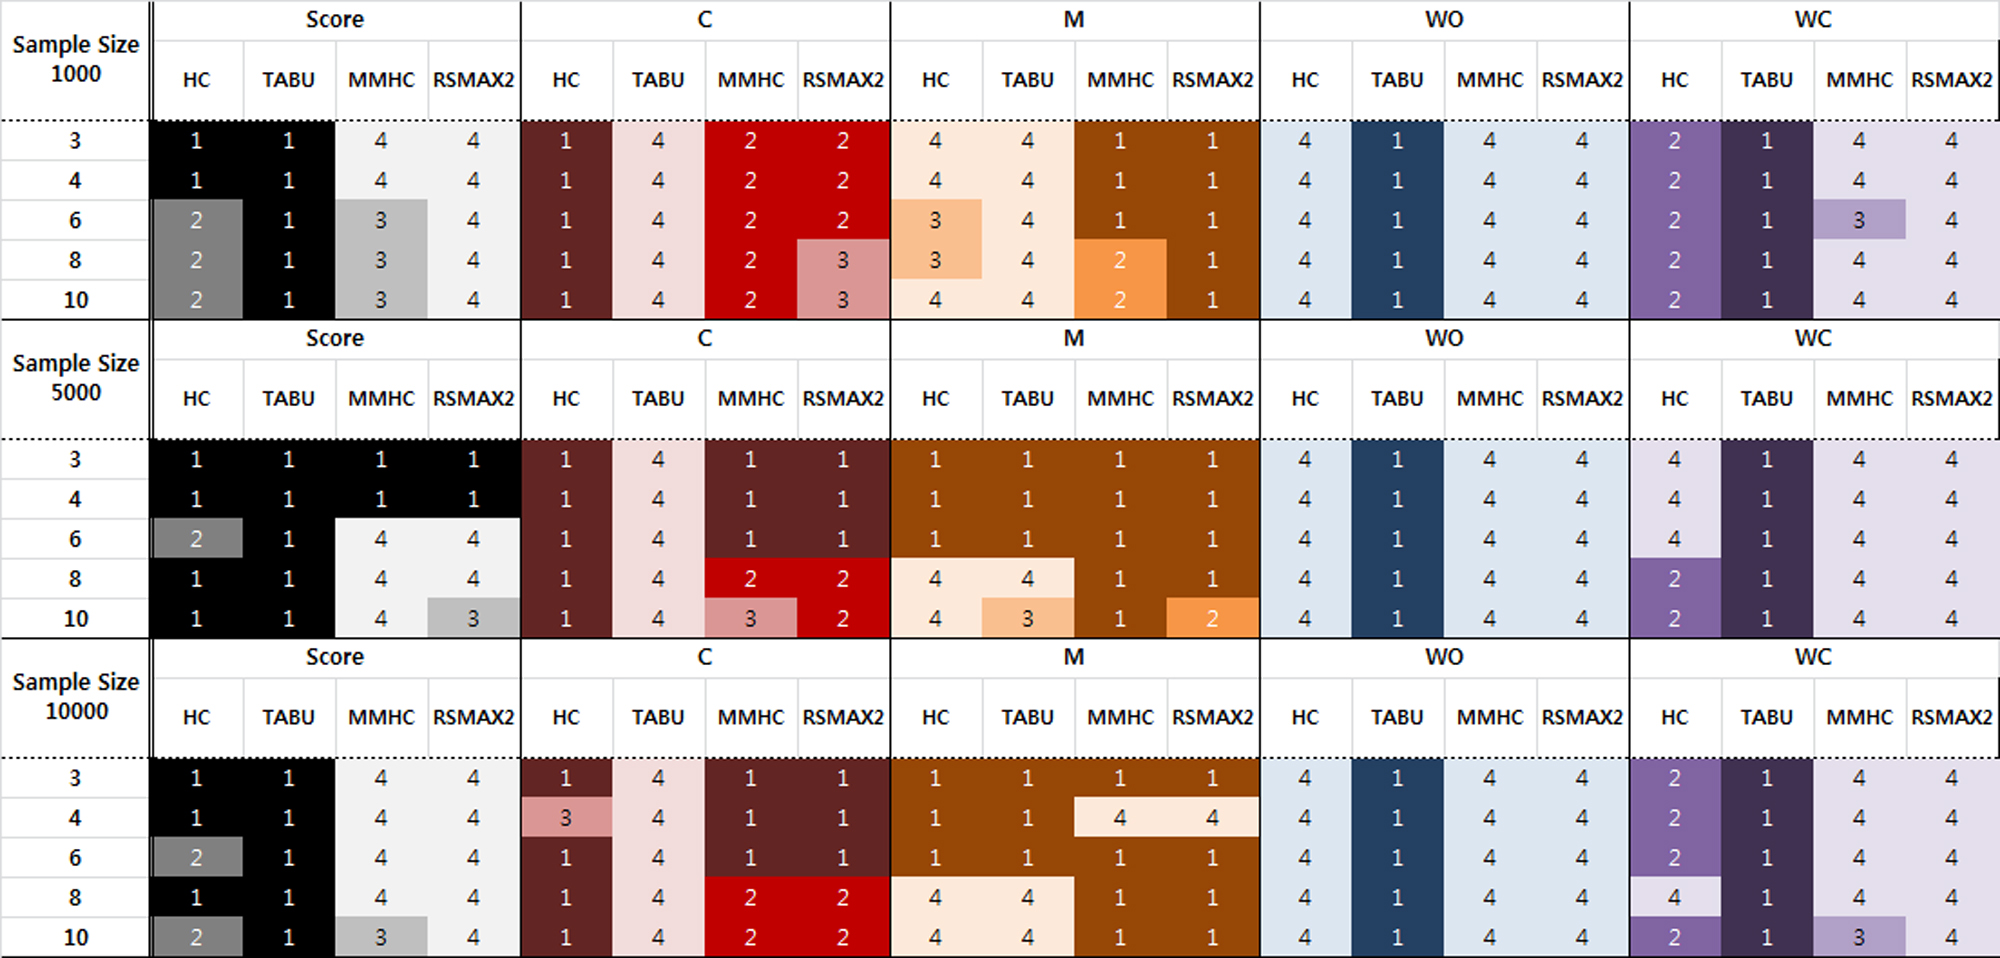
\includegraphics[height=130pt]{images/Result_Line}
	\end{center}
}
\end{frame}



\begin{frame}
\frametitle{Star}
{\scriptsize{}
	\begin{figure}
		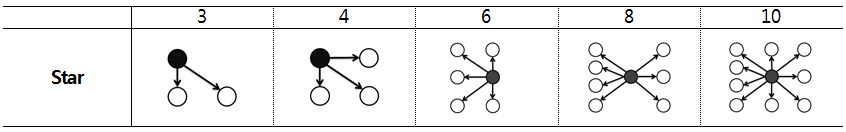
\includegraphics[height=50pt]{images/Topologies_Star}
	\end{figure}	
}
\end{frame}



\begin{frame}
\frametitle{Star (Score)}
{\scriptsize{}
	\begin{figure}
		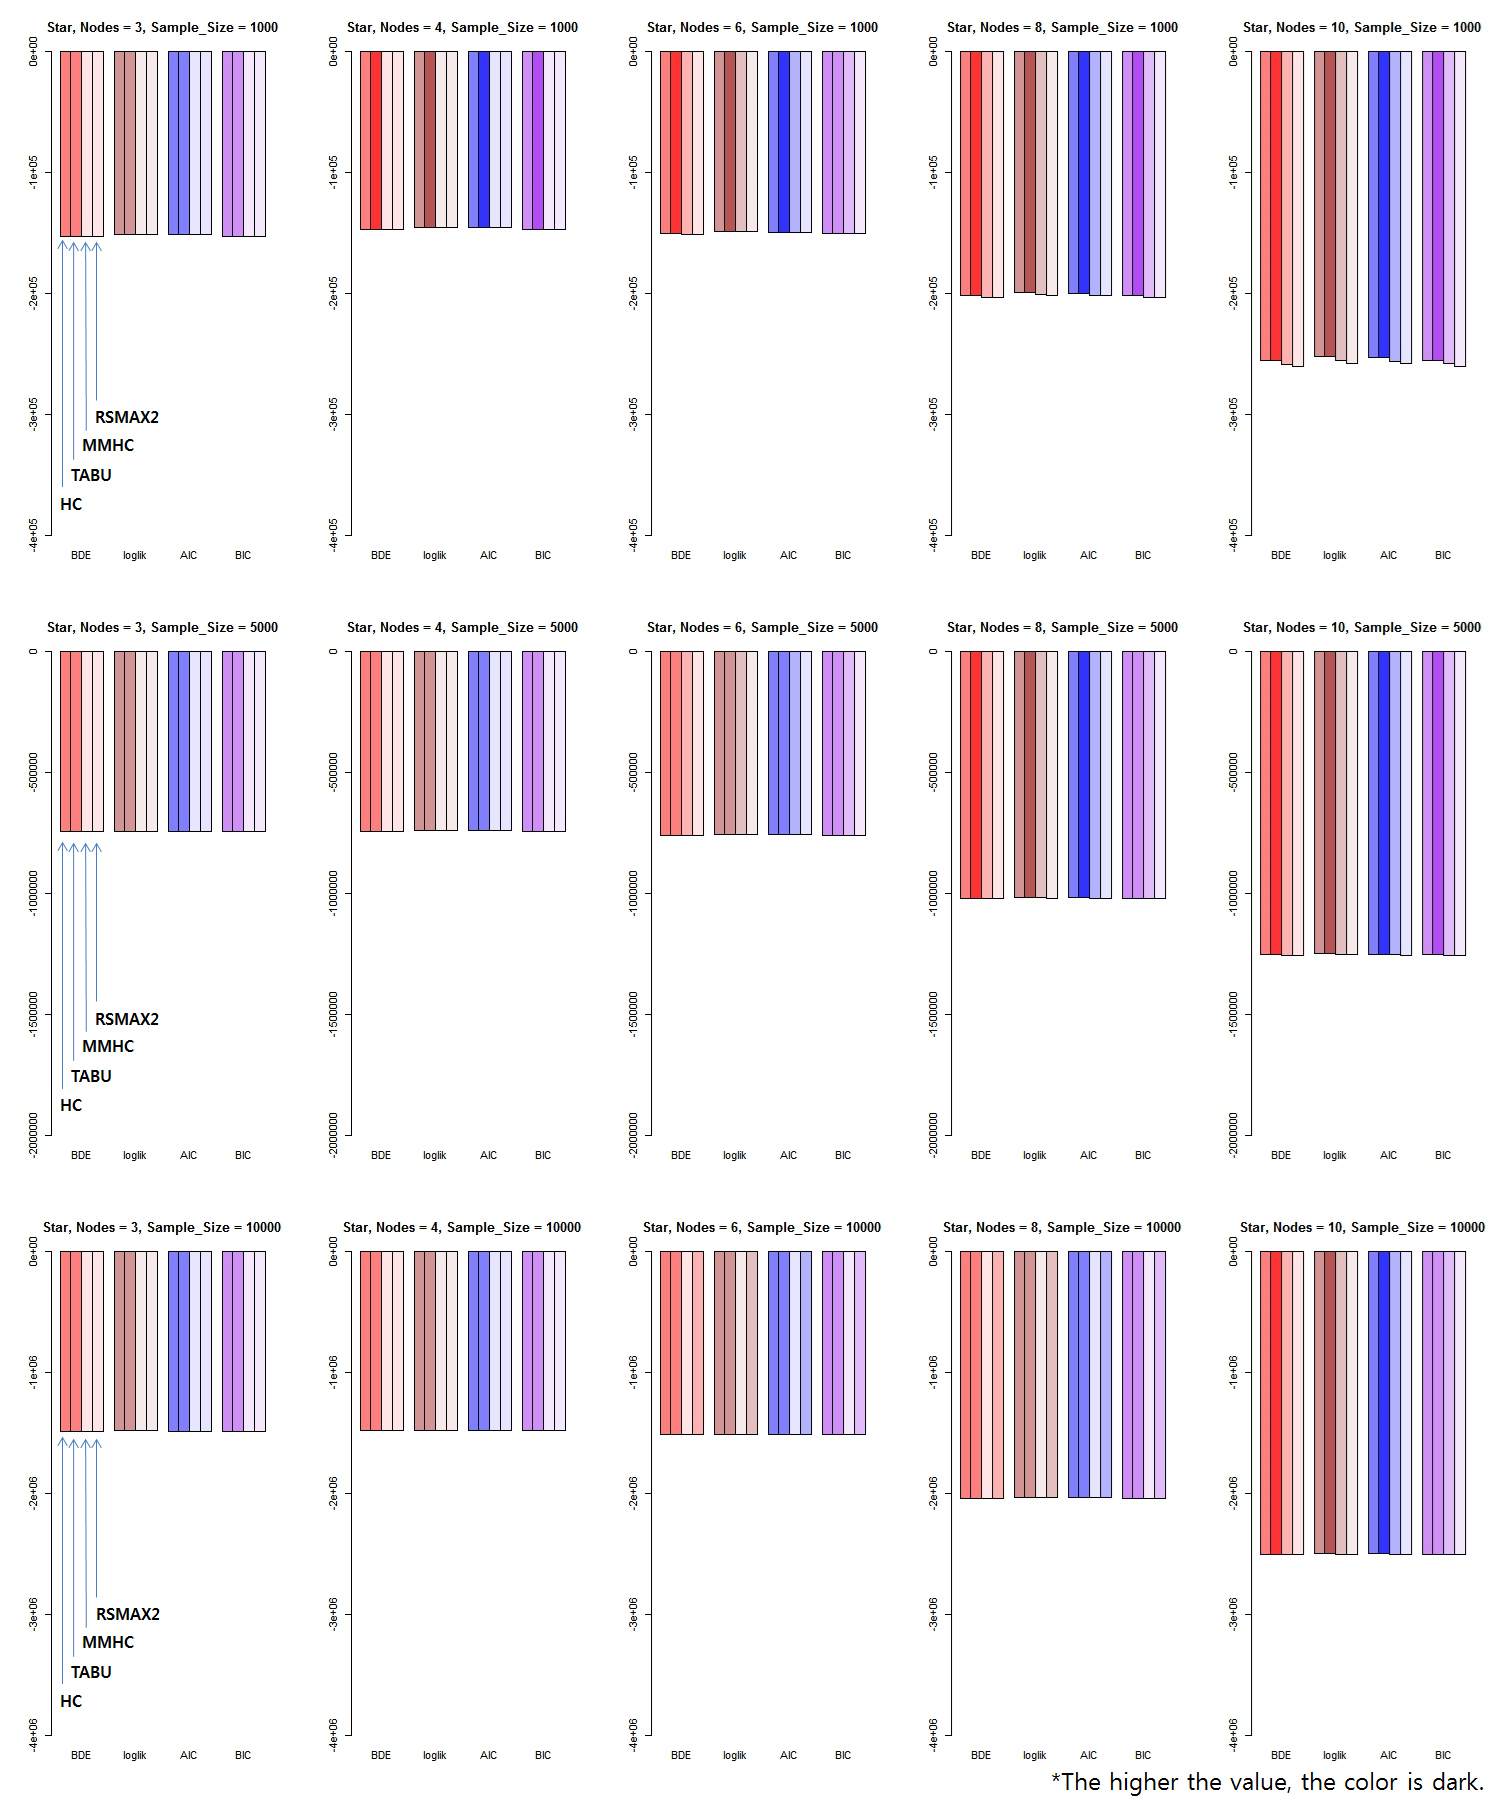
\includegraphics[height=170pt]{images/03_Star_Score}
	\end{figure}	
}
\end{frame}


\begin{frame}
\frametitle{Star (Arcs)}
{\scriptsize{}
	\begin{figure}
		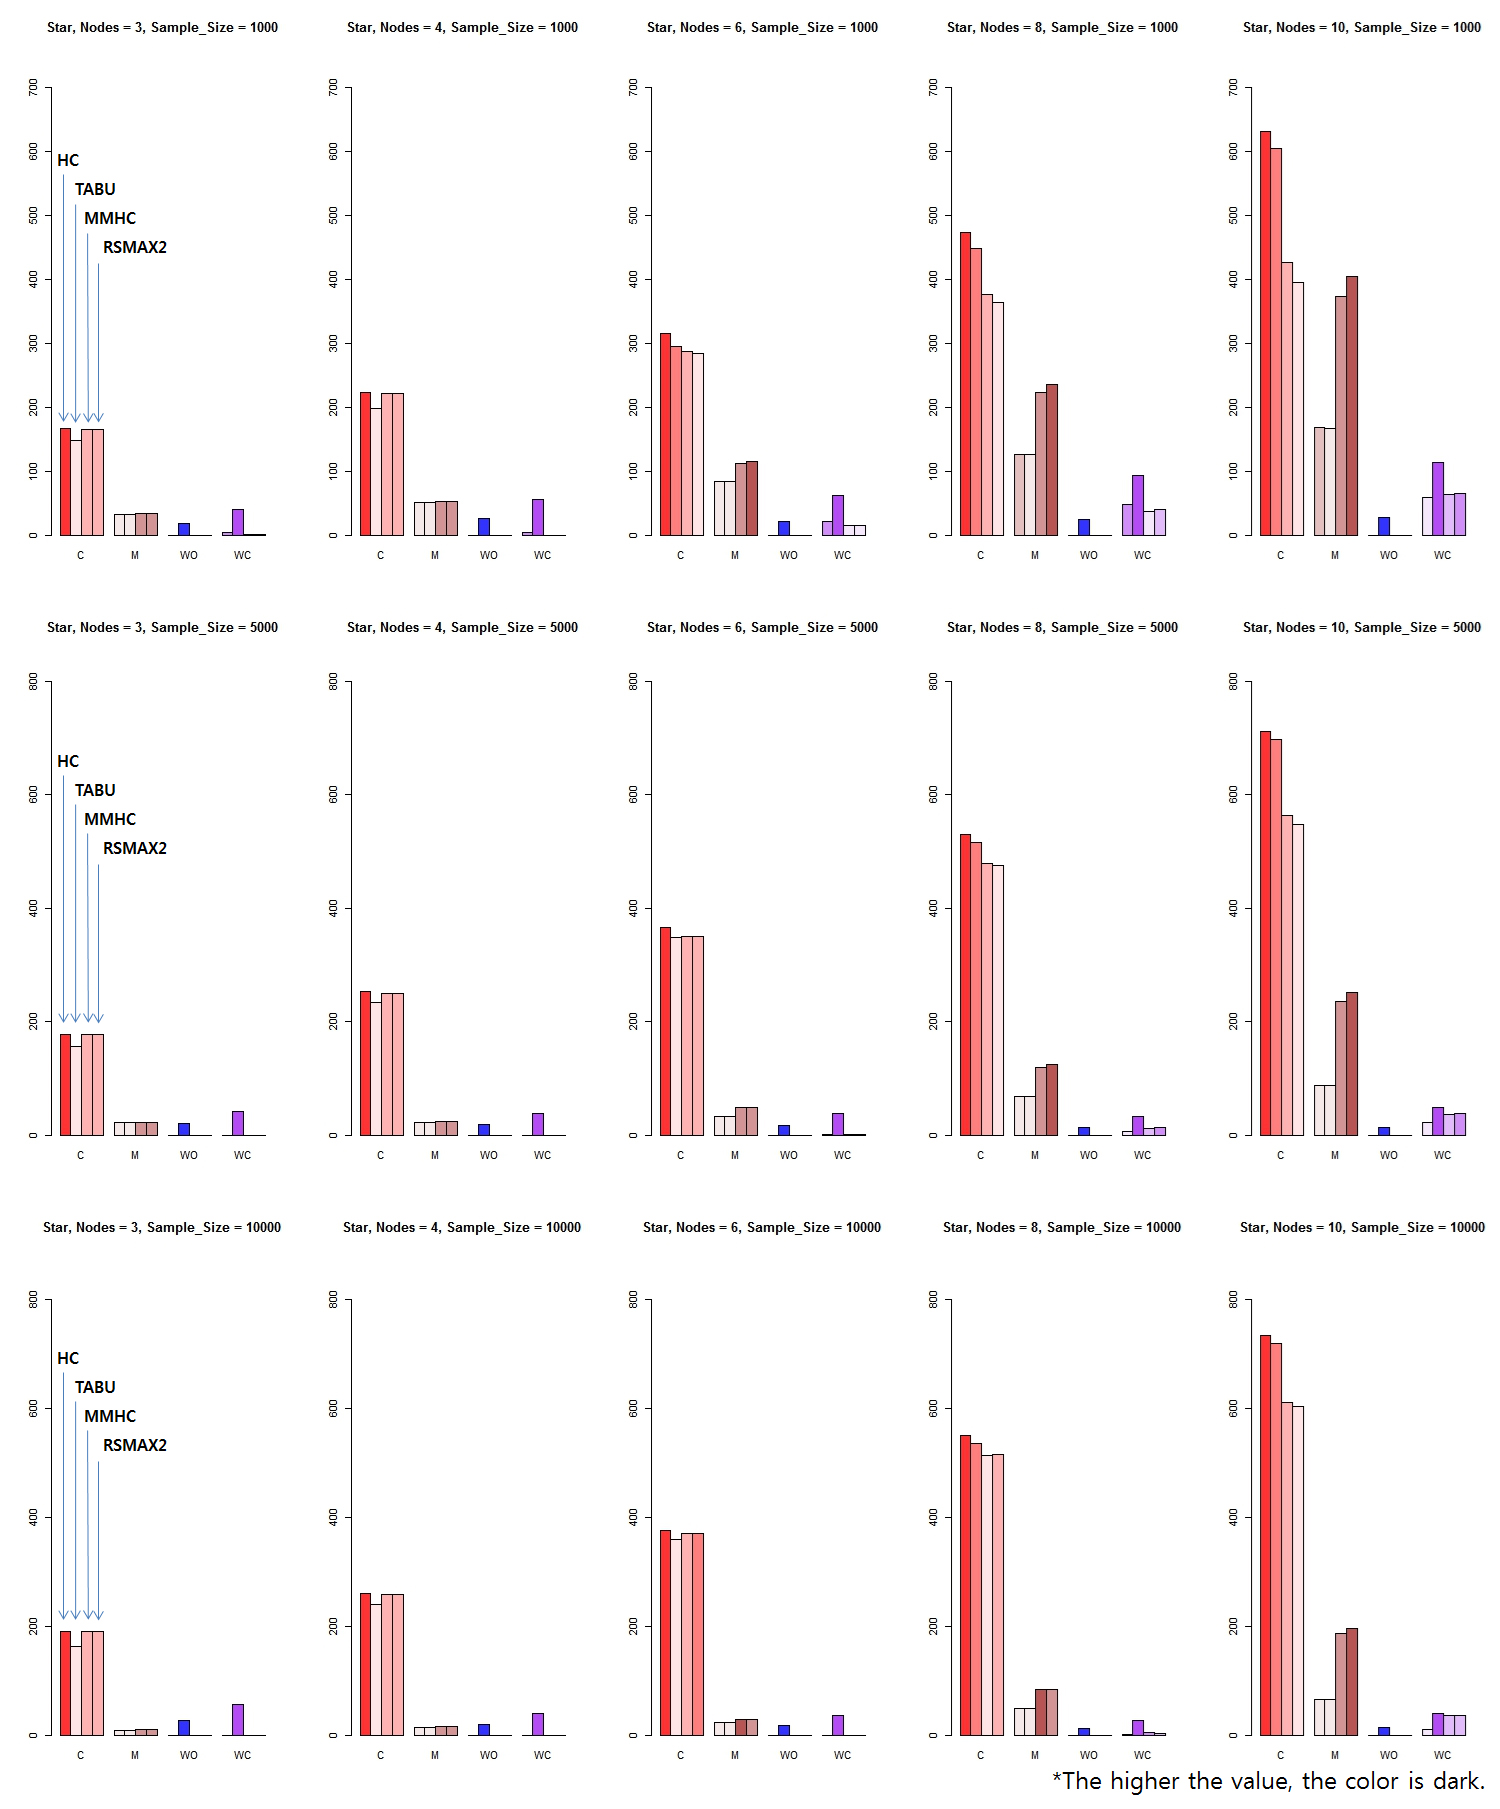
\includegraphics[height=170pt]{images/03_Star_Arcs}
	\end{figure}	
}
\end{frame}



\begin{frame}
\frametitle{Star}
{\scriptsize{}
	\begin{center}
		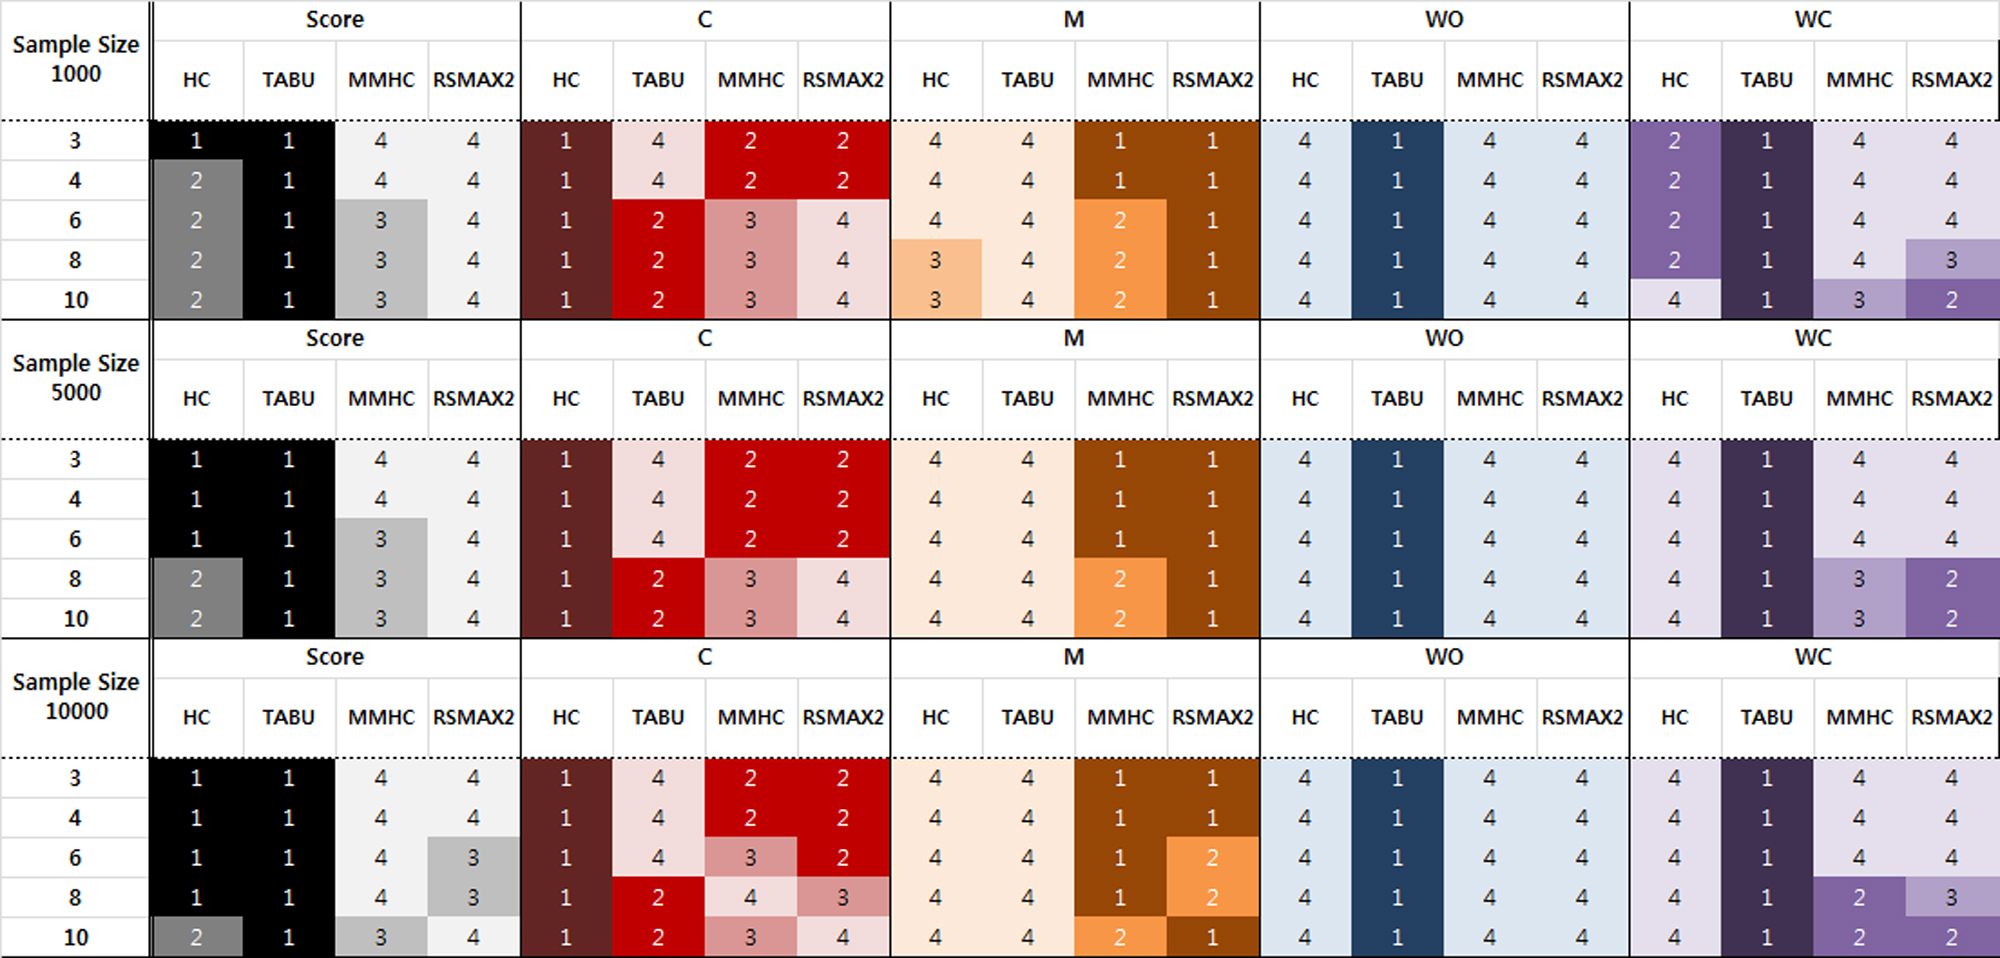
\includegraphics[height=130pt]{images/Result_Star}
	\end{center}
}
\end{frame}



\begin{frame}
\frametitle{PseudoLoop}
{\scriptsize{}
	\begin{figure}
		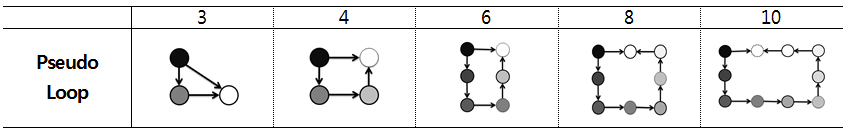
\includegraphics[height=50pt]{images/Topologies_PseudoLoop}
	\end{figure}	
}
\end{frame}



\begin{frame}
\frametitle{PseudoLoop (Score)}
{\scriptsize{}
	\begin{figure}
		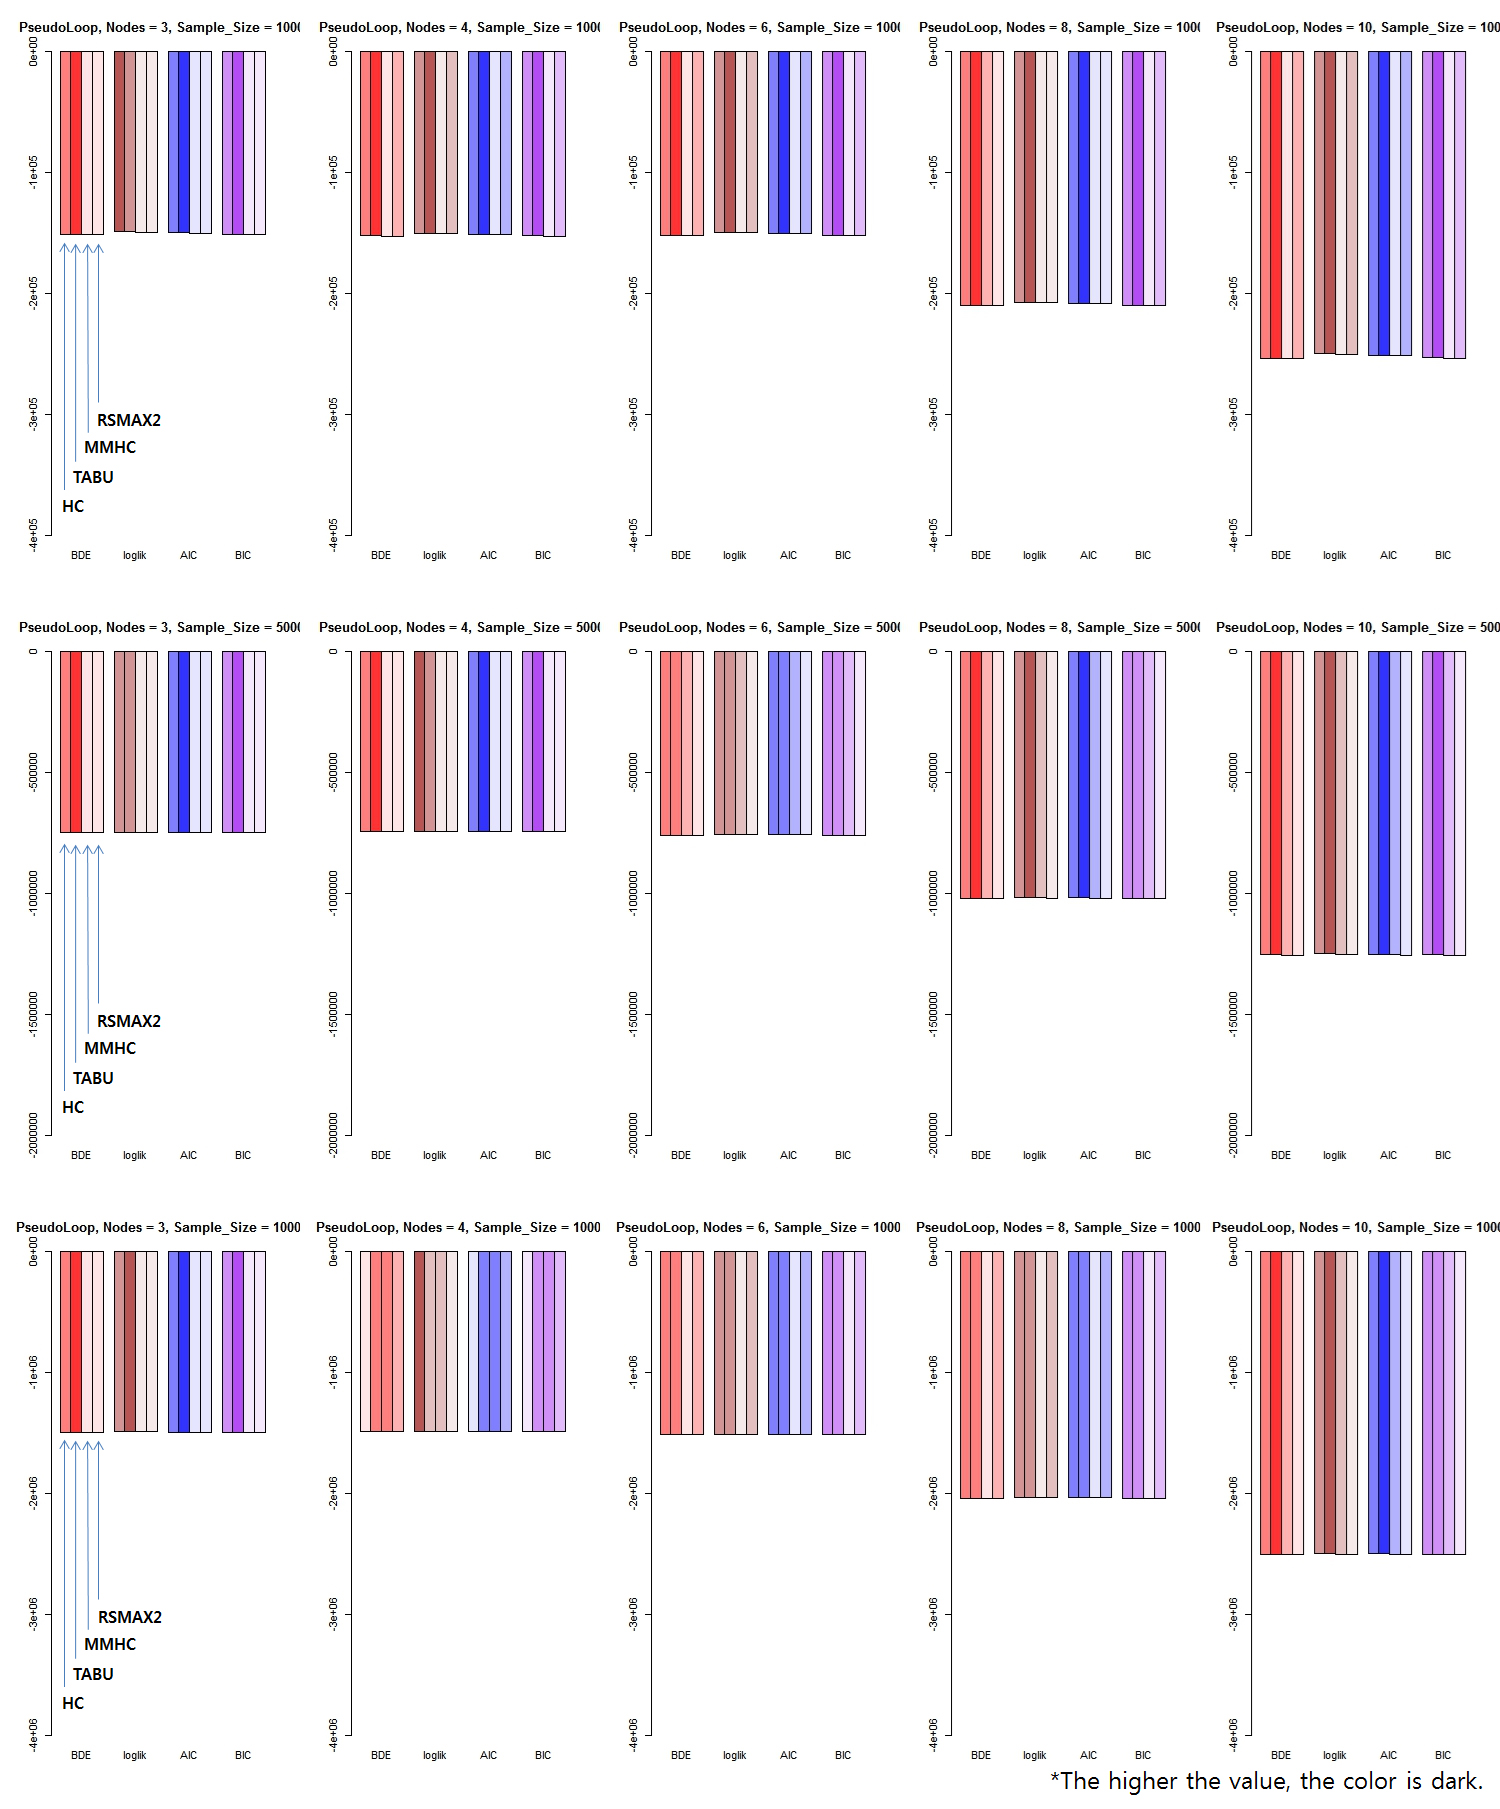
\includegraphics[height=170pt]{images/04_PseudoLoop_Score}
	\end{figure}	
}
\end{frame}


\begin{frame}
\frametitle{PseudoLoop (Arc)}
{\scriptsize{}
	\begin{figure}
		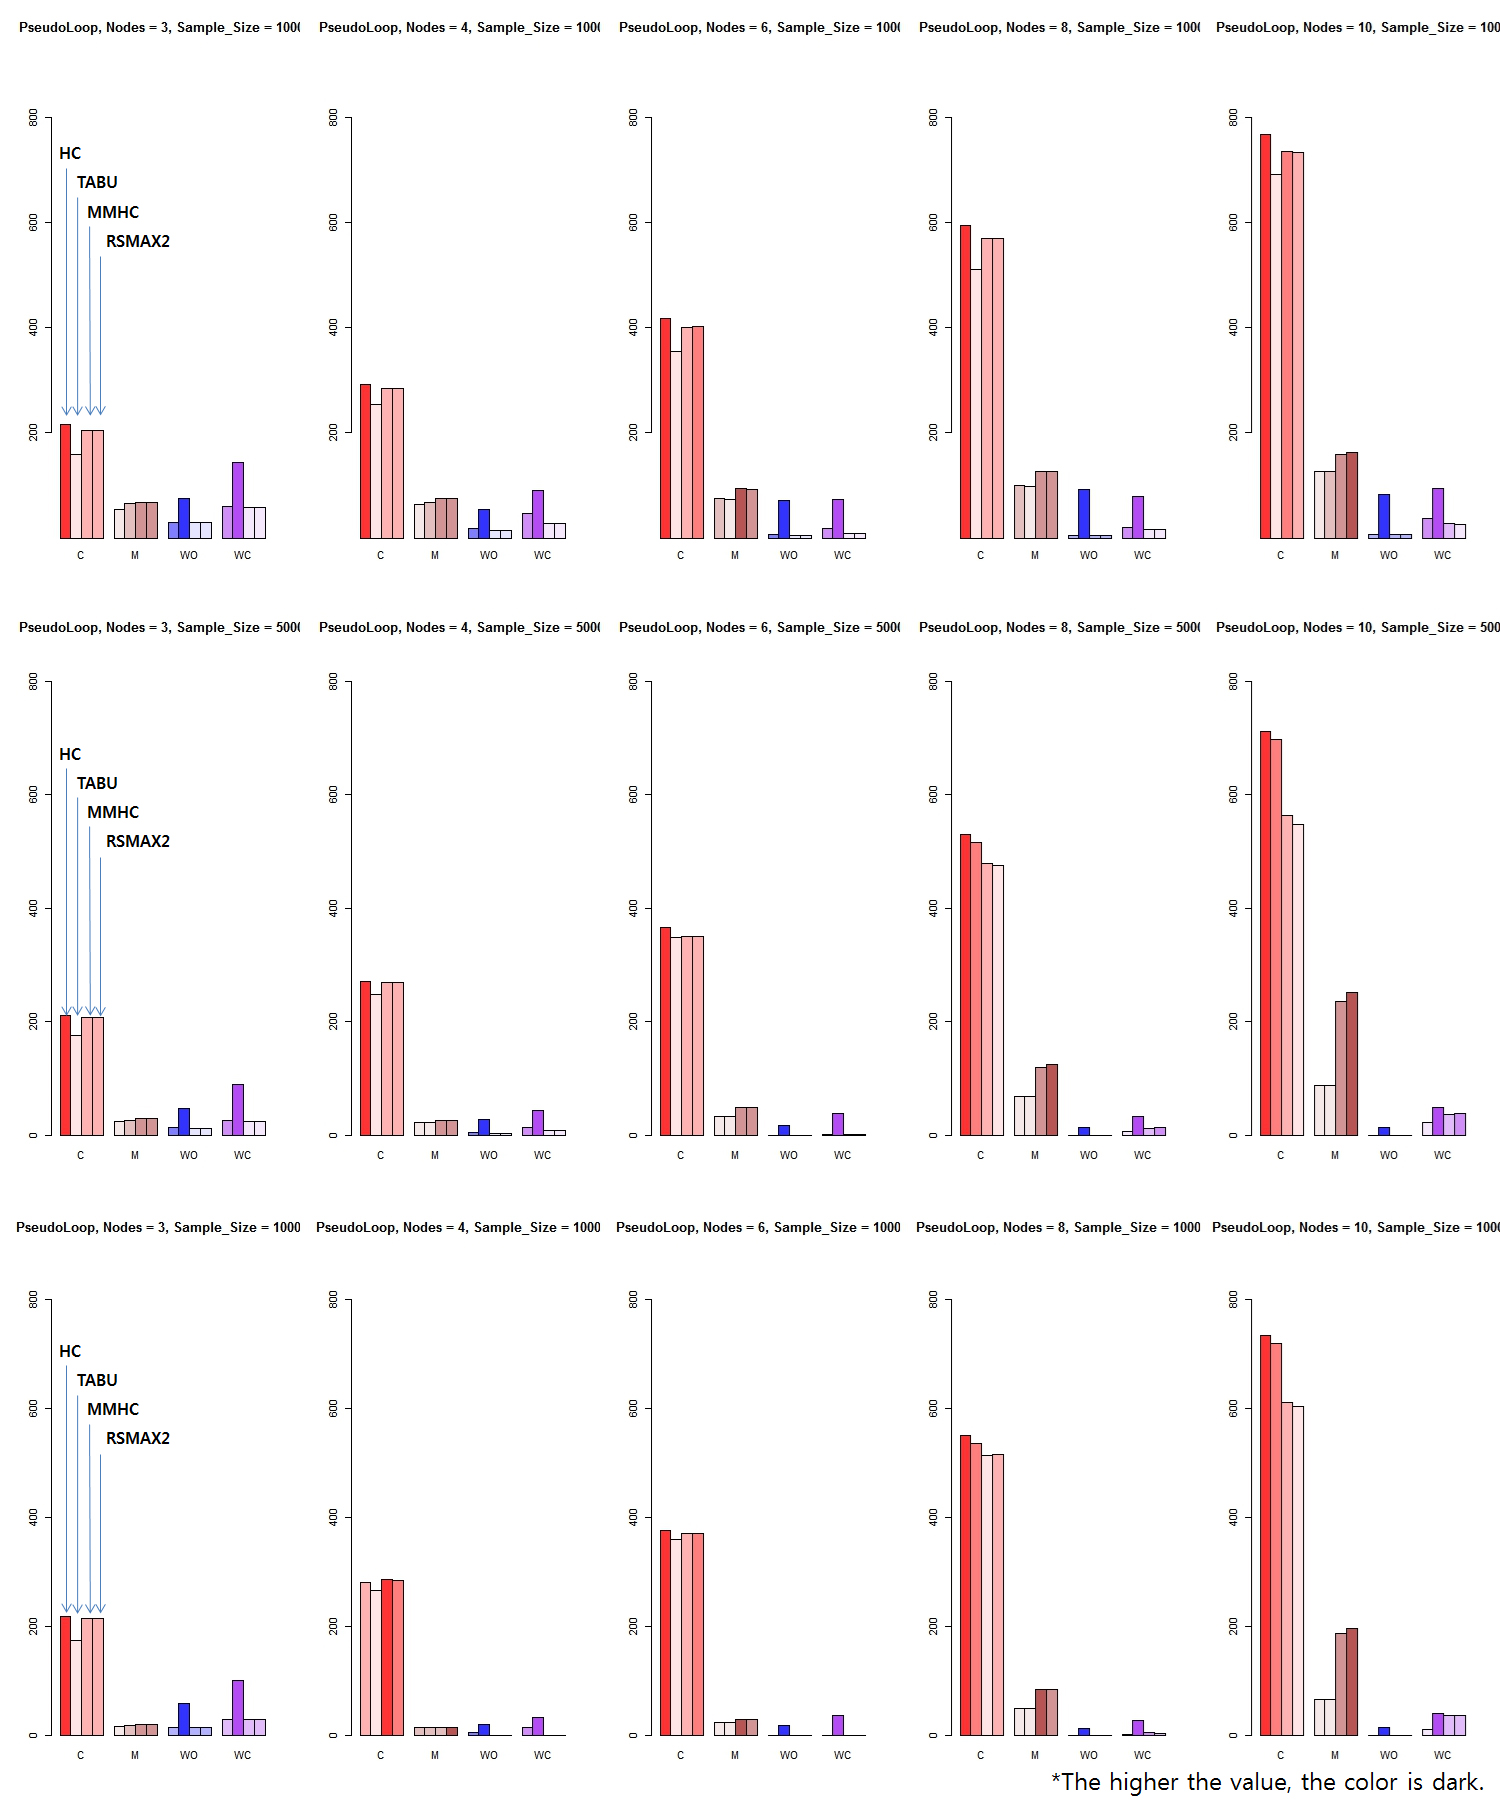
\includegraphics[height=170pt]{images/04_PseudoLoop_Arcs}
	\end{figure}	
}
\end{frame}


\begin{frame}
\frametitle{PseudoLoop}
{\scriptsize{}
	\begin{center}
		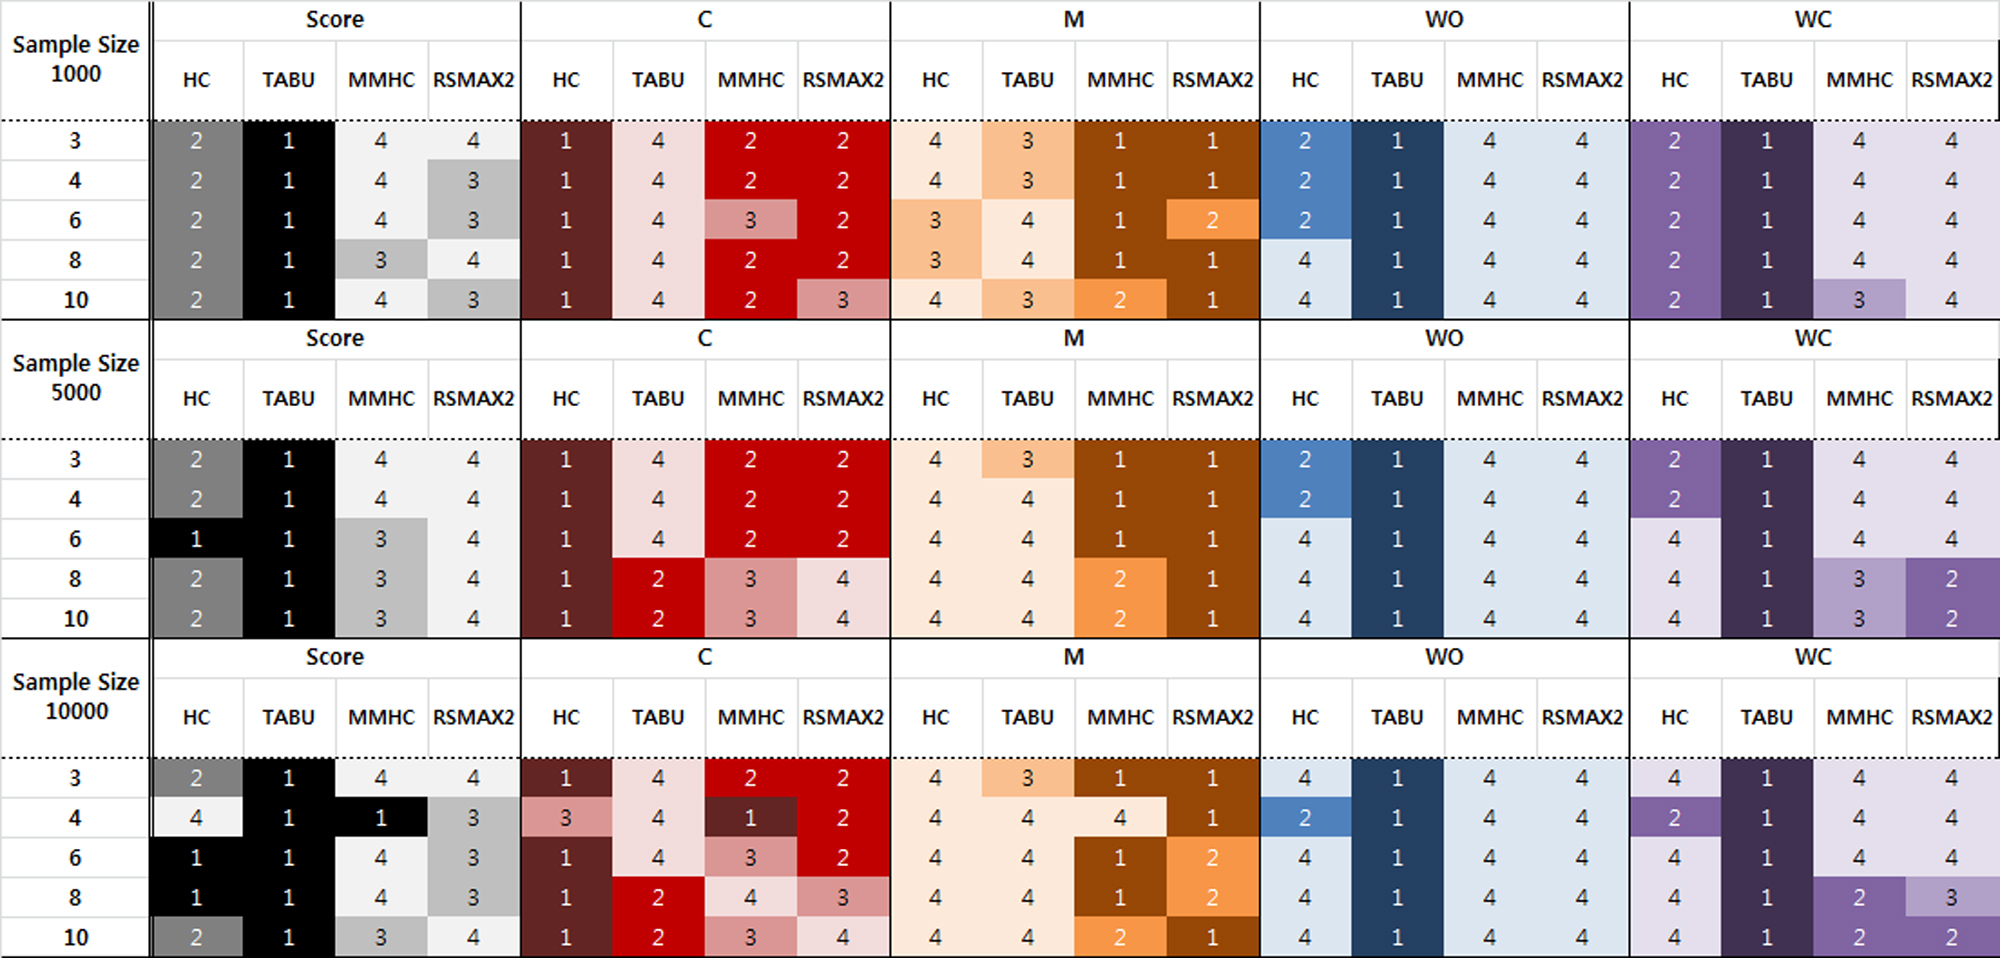
\includegraphics[height=130pt]{images/Result_PseudoLoop}
	\end{center}
}
\end{frame}




\begin{frame}
\frametitle{Diamond}
{\scriptsize{}
	\begin{figure}
		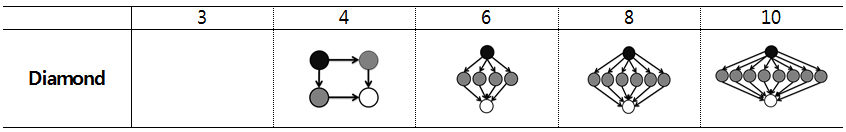
\includegraphics[height=50pt]{images/Topologies_Diamond}
	\end{figure}	
}
\end{frame}



\begin{frame}
\frametitle{Diamond (Score)}
{\scriptsize{}
	\begin{figure}
		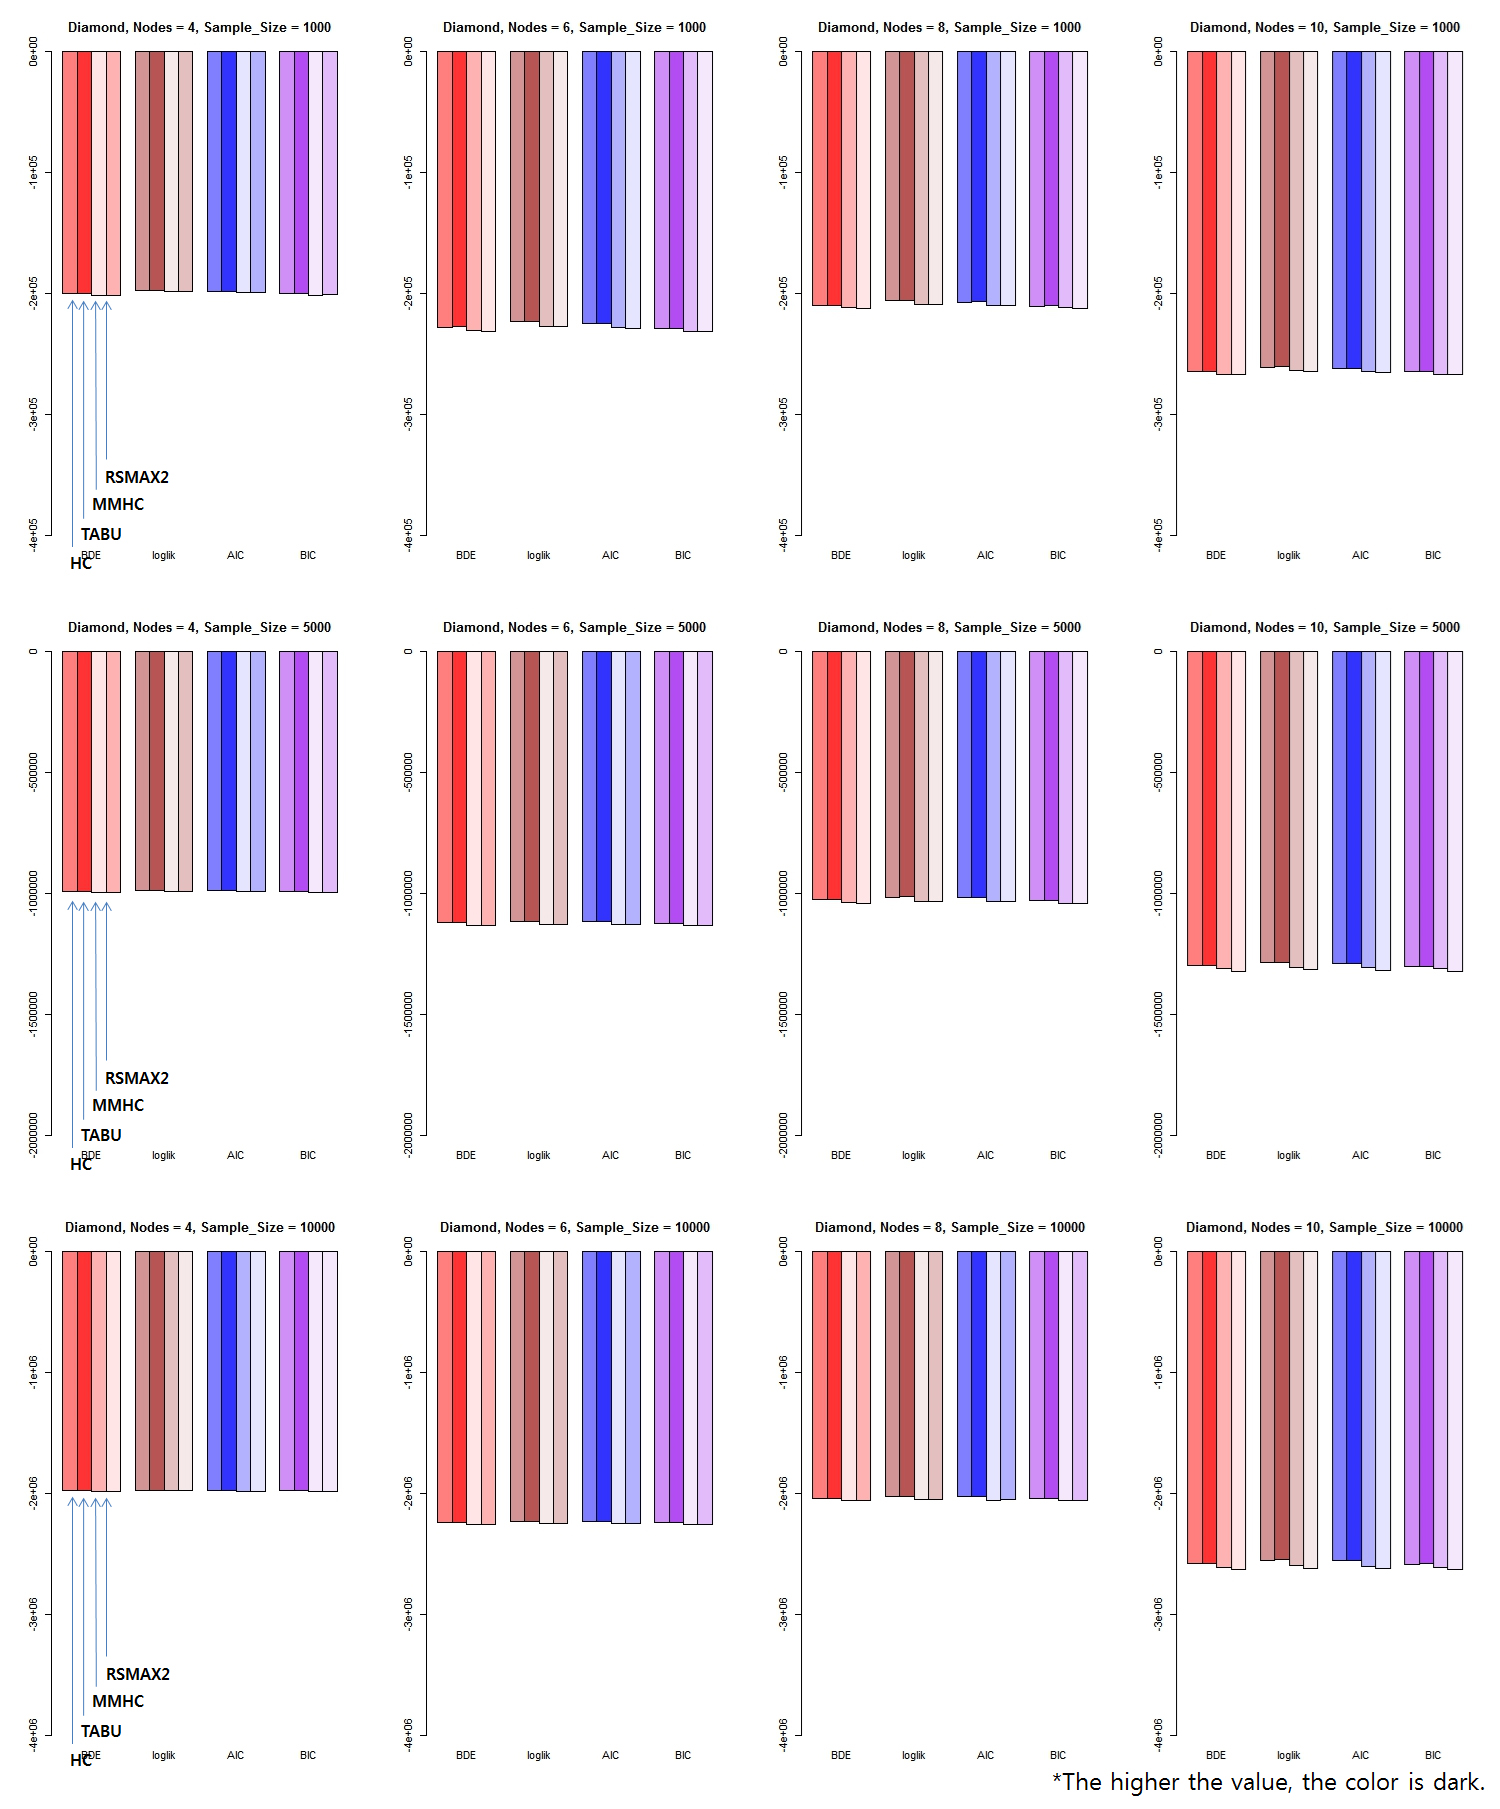
\includegraphics[height=170pt]{images/05_Diamond_Score}
	\end{figure}	
}
\end{frame}


\begin{frame}
\frametitle{Diamond (Arc)}
{\scriptsize{}
	\begin{figure}
		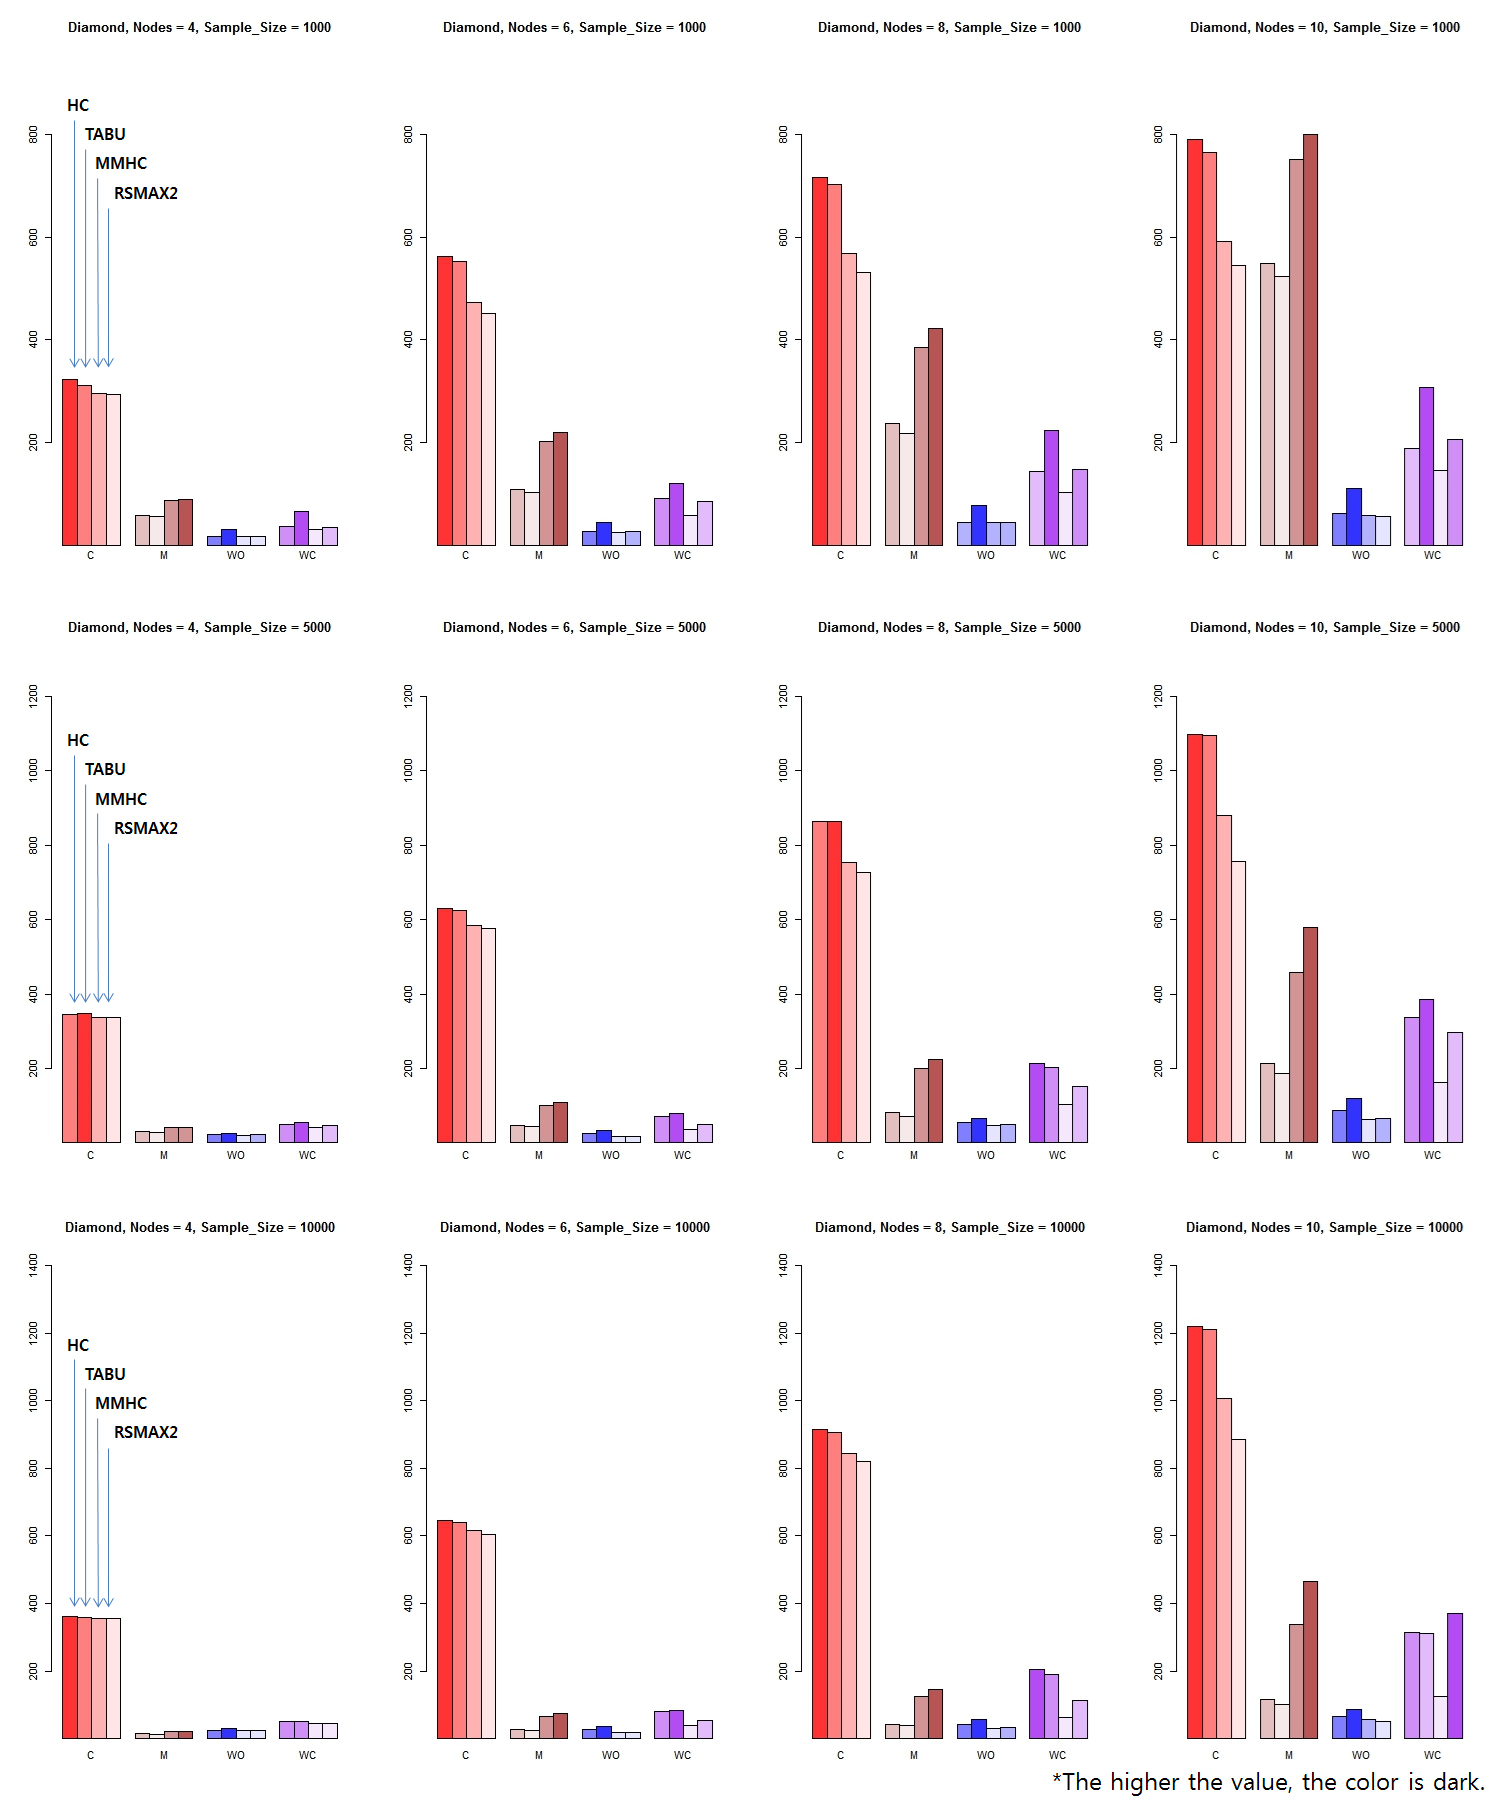
\includegraphics[height=170pt]{images/05_Diamond_Arcs}
	\end{figure}	
}
\end{frame}


\begin{frame}
\frametitle{Diamond}
{\scriptsize{}
	\begin{center}
		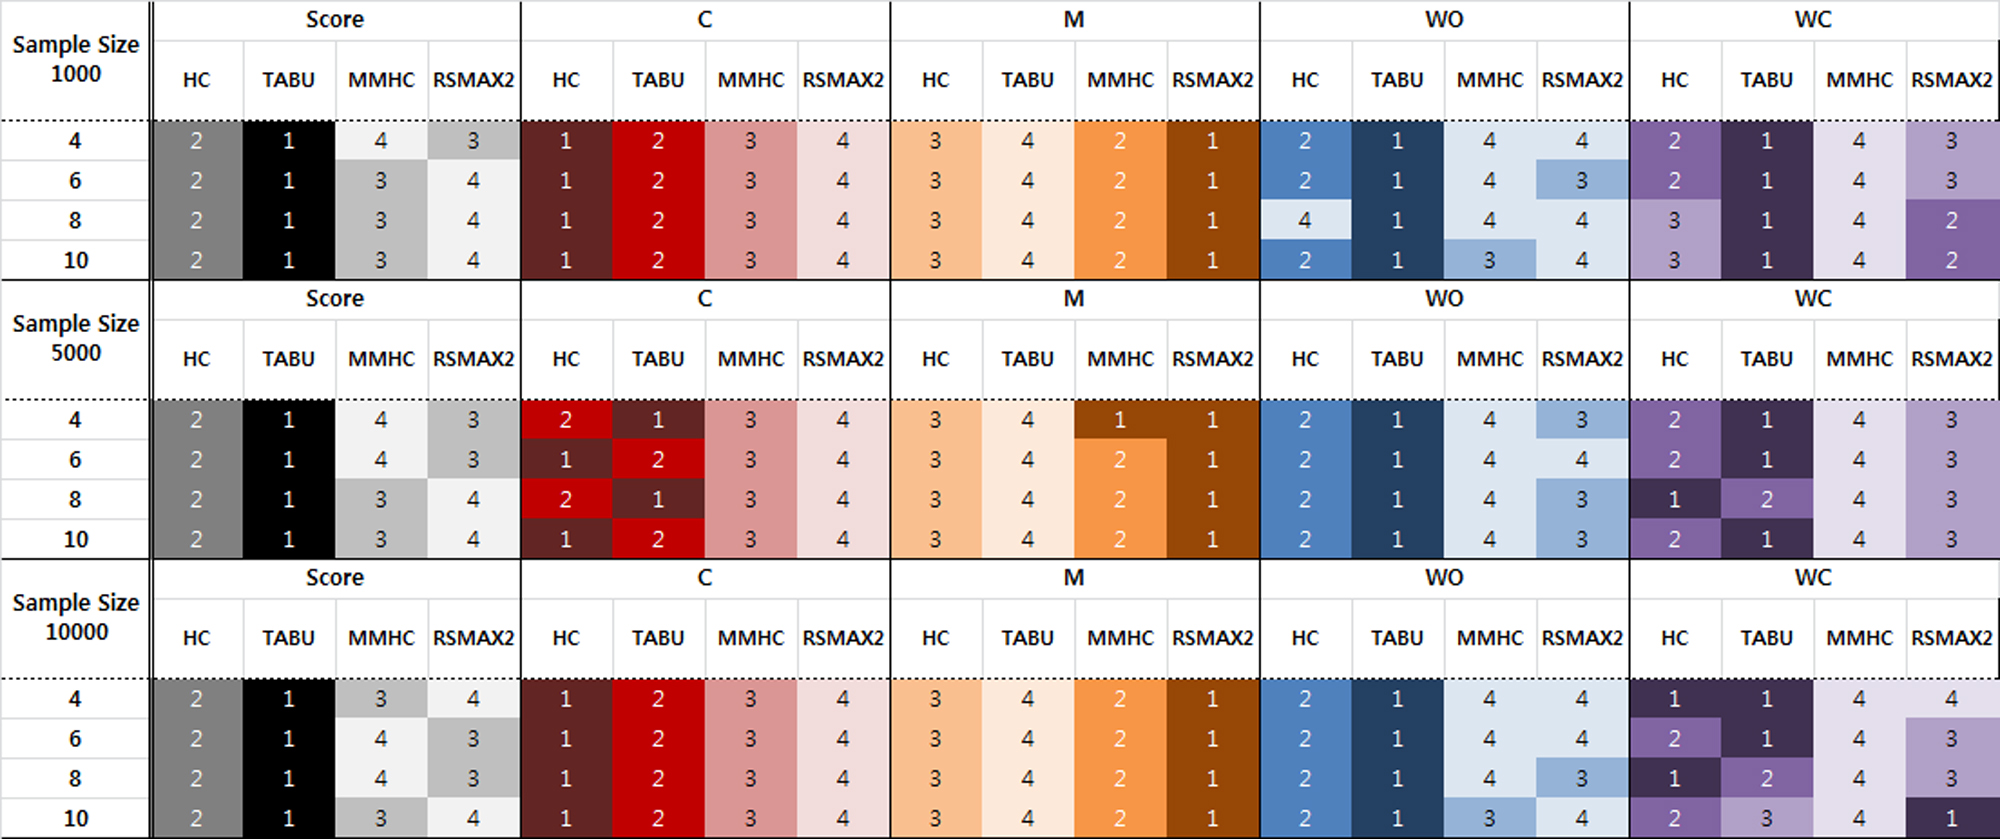
\includegraphics[height=130pt]{images/Result_Diamond}
	\end{center}
}
\end{frame}


\begin{frame}
\frametitle{Rhombus}
{\scriptsize{}
	\begin{figure}
		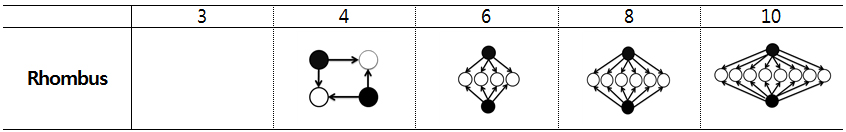
\includegraphics[height=50pt]{images/Topologies_Rhombus}
	\end{figure}	
}
\end{frame}



\begin{frame}
\frametitle{Rhombus (Score)}
{\scriptsize{}
	\begin{figure}
		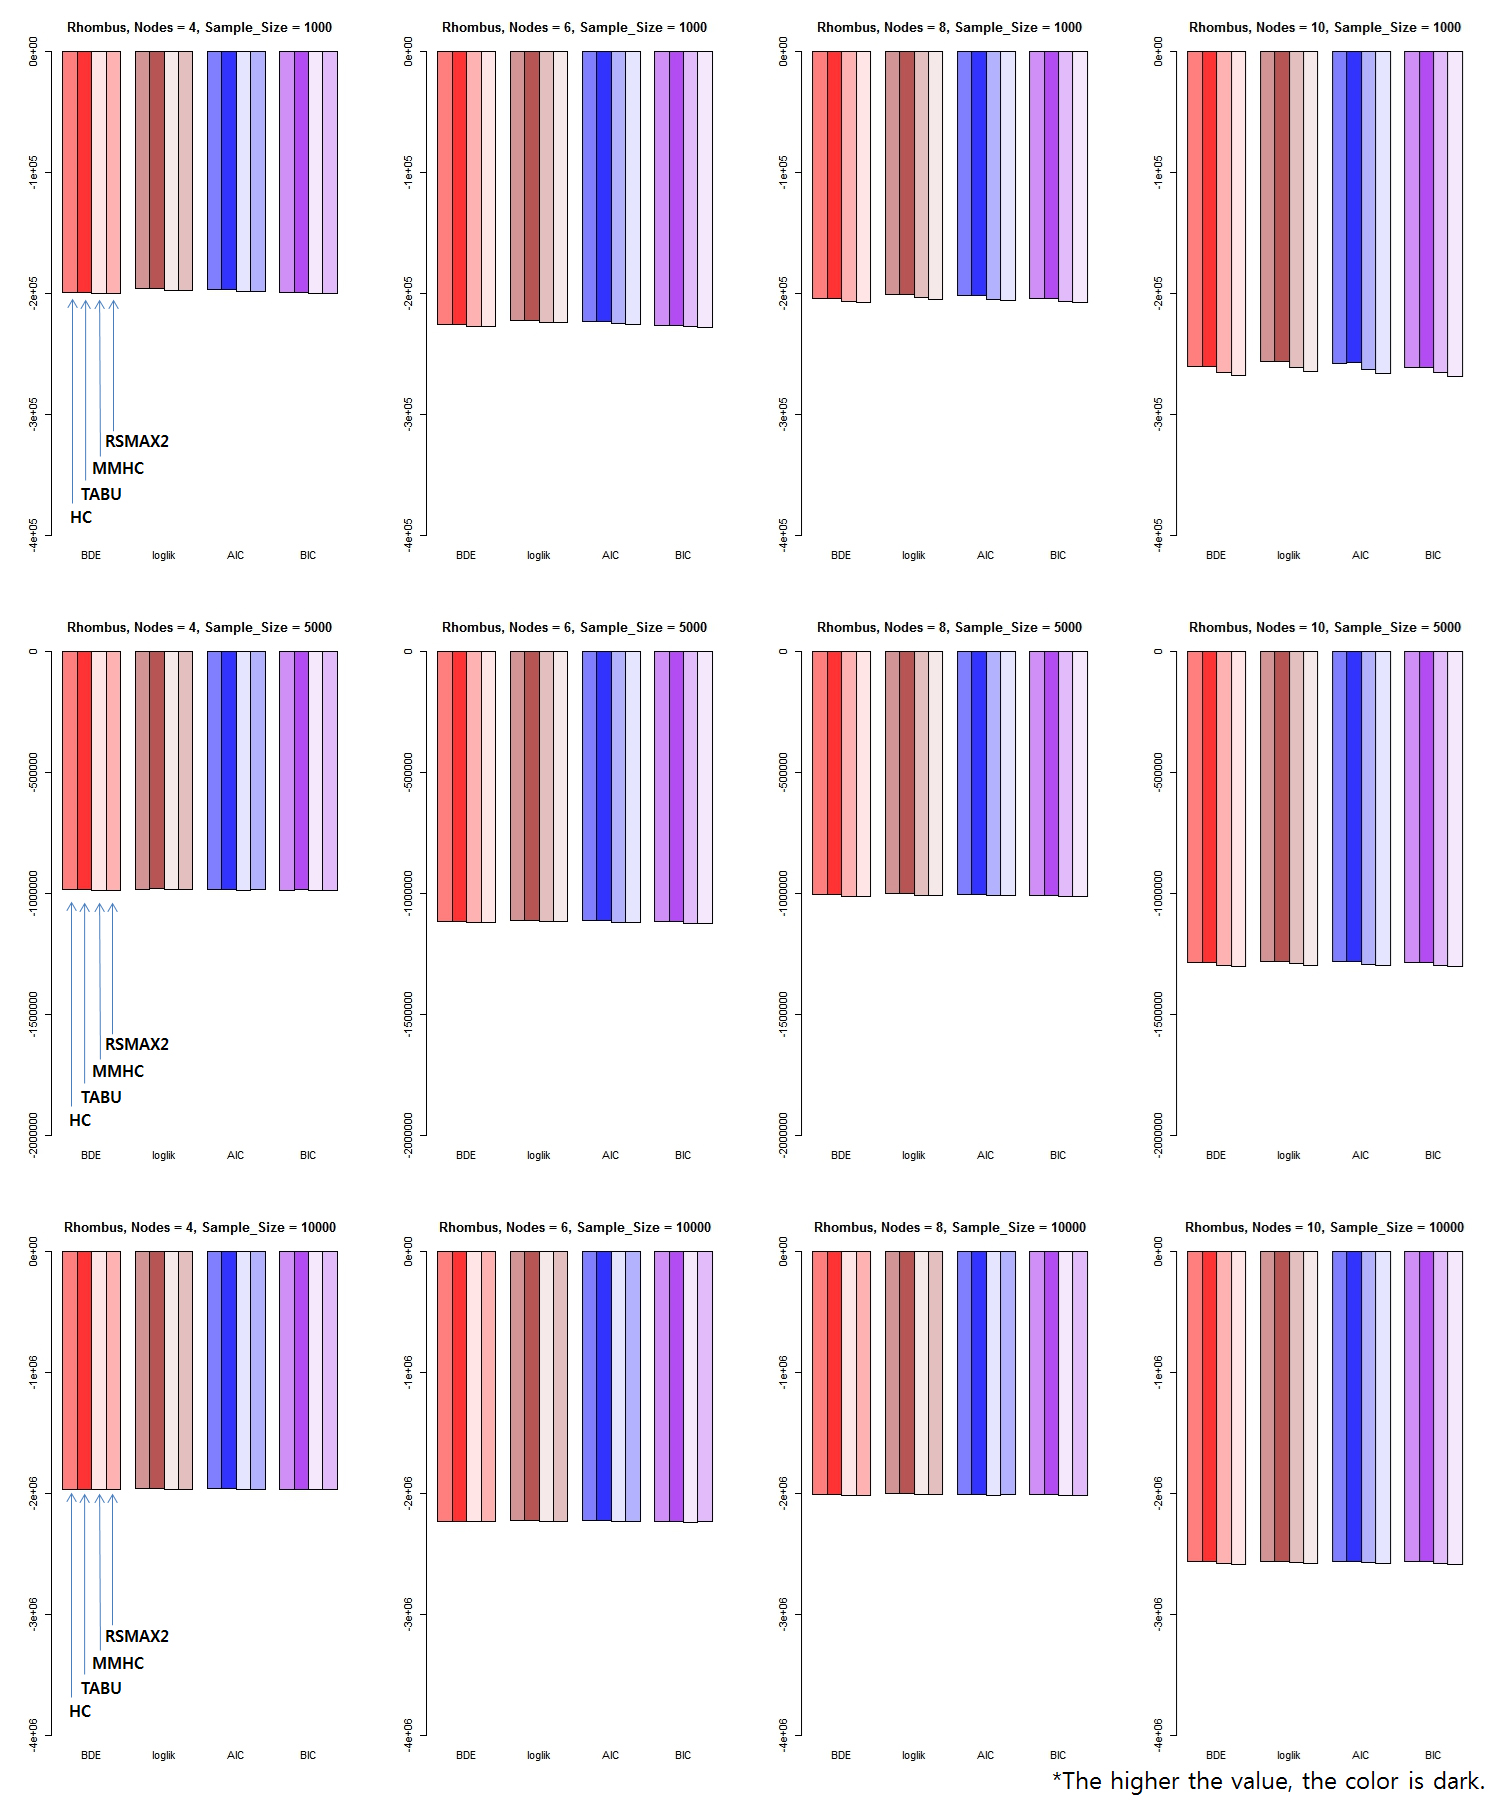
\includegraphics[height=170pt]{images/06_Rhombus_Score}
	\end{figure}	
}
\end{frame}


\begin{frame}
\frametitle{Rhombus (Arc)}
{\scriptsize{}
	\begin{figure}
		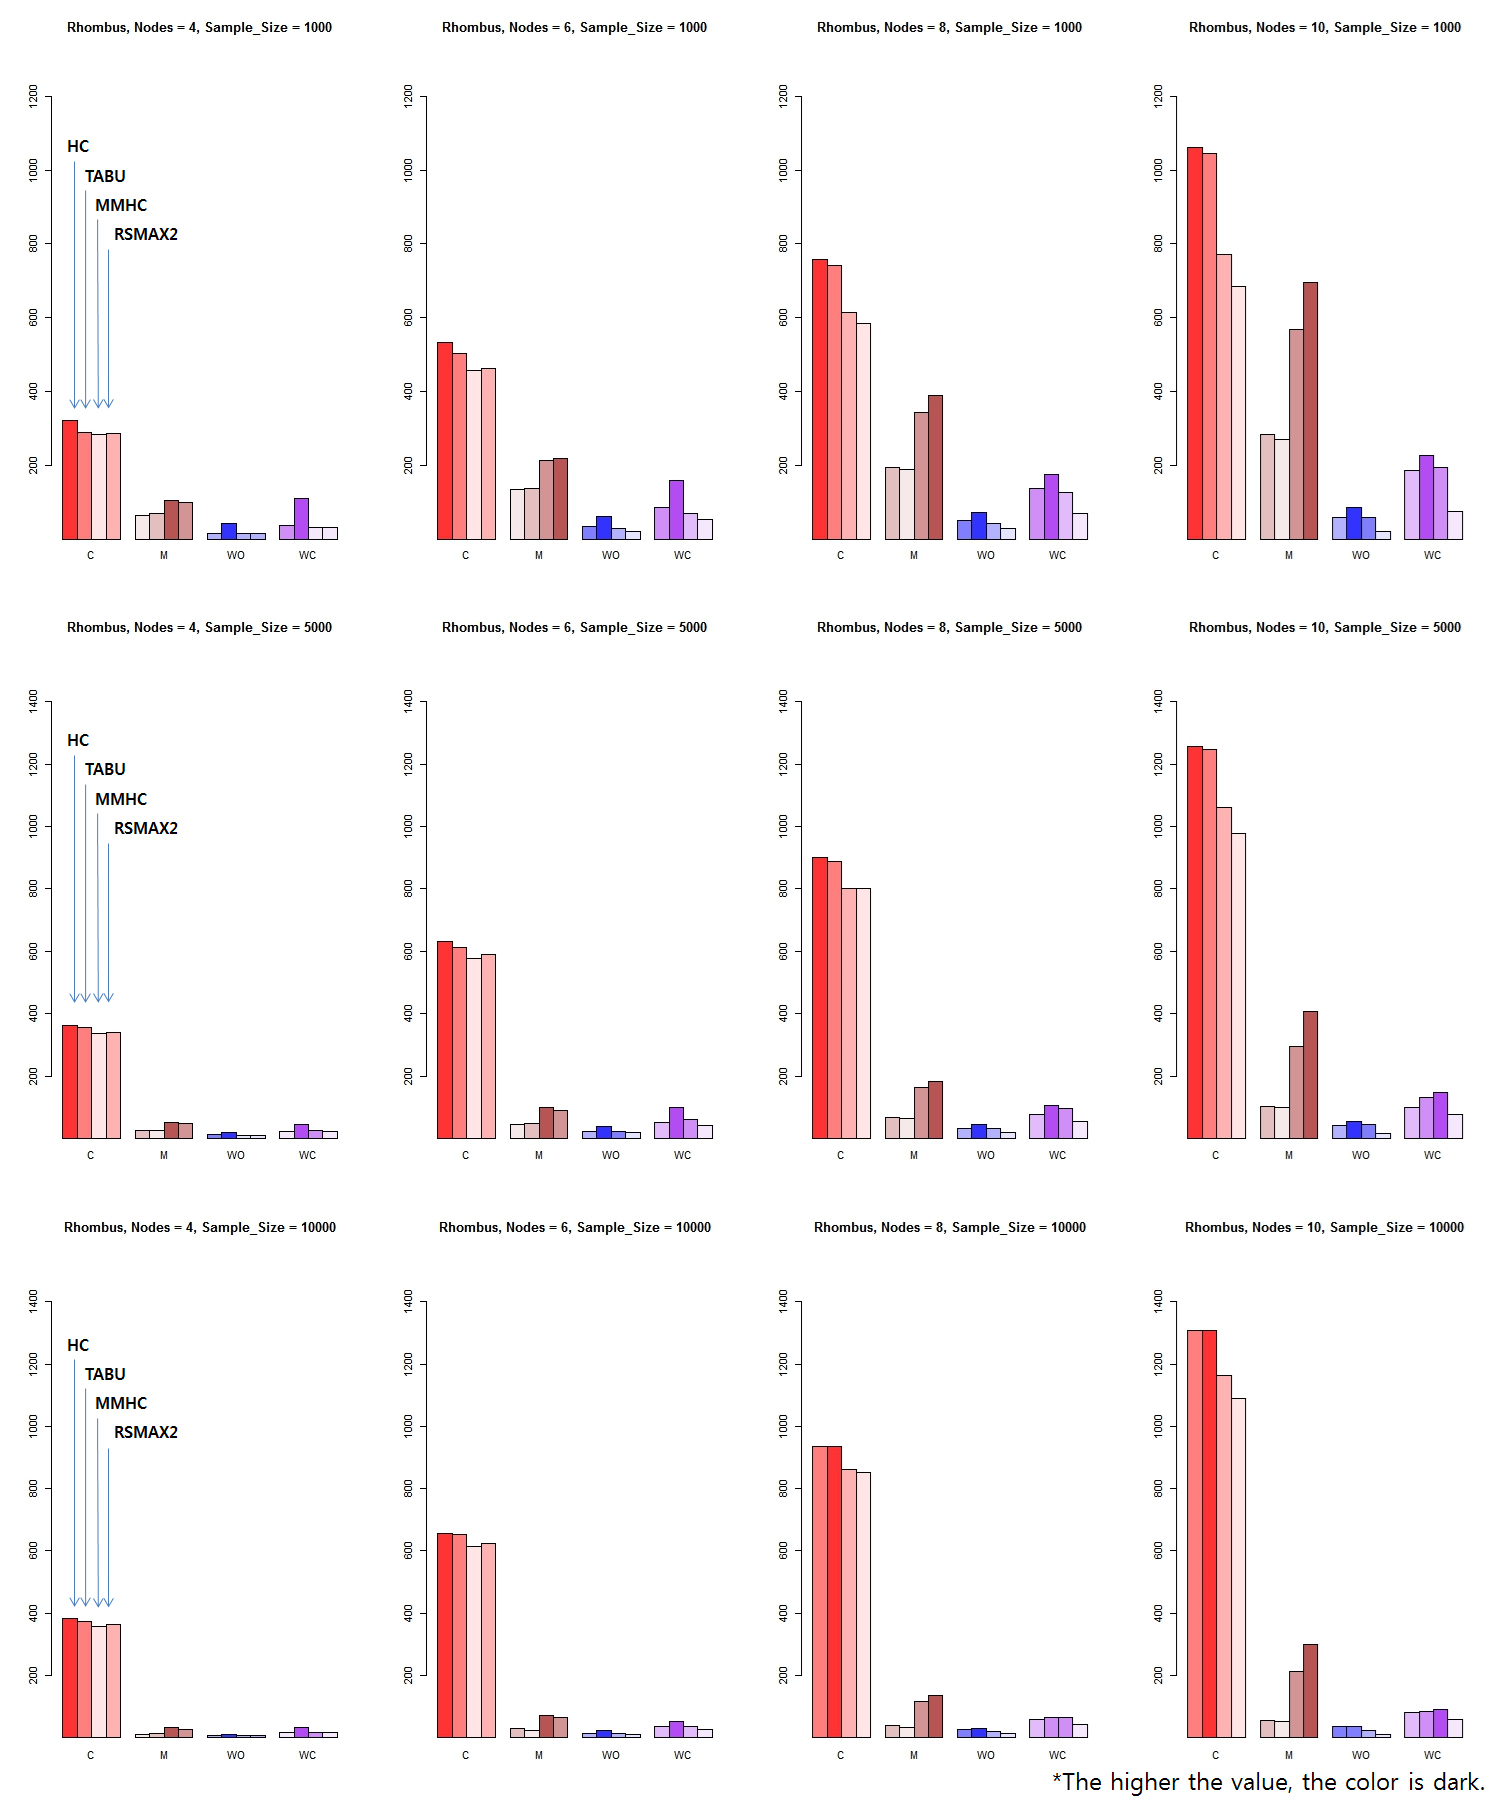
\includegraphics[height=170pt]{images/06_Rhombus_Arcs}
	\end{figure}	
}
\end{frame}



\begin{frame}
\frametitle{Rhombus}
{\scriptsize{}
	\begin{center}
		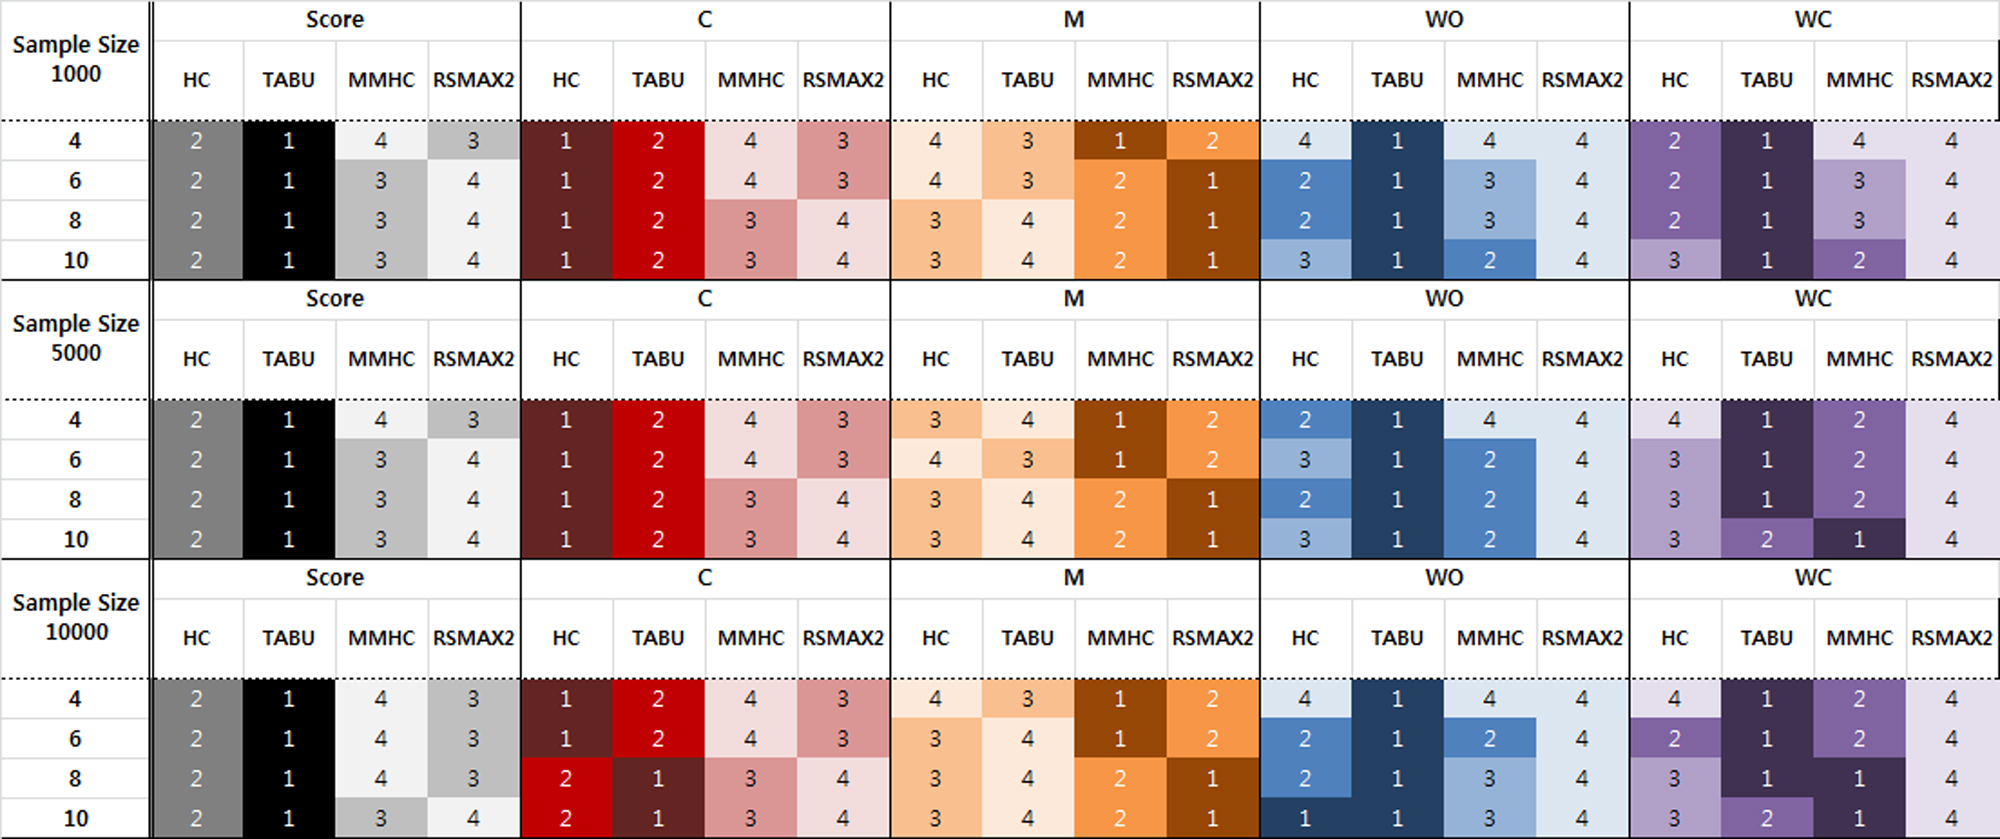
\includegraphics[height=130pt]{images/Result_Rhombus}
	\end{center}
}
\end{frame}



\section{Discussion}
\begin{frame}
\frametitle{Discussion}
{\scriptsize{}
	\begin{itemize}
	\item In most cases using synthetic data according to topology,
	
	If \textcolor{red}{comparing by score}, then \textcolor{red}{TABU search} has good performance.
	
	But \textcolor{red}{comparing by reference to "What C is the lot?"}, then \textcolor{red}{HC} has also good performance.
	
	{}\	
	
	\item \textcolor{red}{Hybrid algorithm} compared to Score-based algorithm is found to be that \textcolor{red}{draw the arc more conservative}.

	{}\
	
	\item  \textcolor{red}{Sample size is larger}, then C was increased.
	
	In addition, M, WO and WC was decreased.
	
	{}\

	\item About  \textcolor{red}{Line} and  \textcolor{red}{Star} form, the performance difference due to relatively algorithm was not large compared to other topology.
	\end{itemize}
}
\end{frame}
\end{document}